\documentclass[journal]{IEEEtran}
\usepackage[a5paper, margin=10mm]{geometry}
%\usepackage{lmodern} % Ensure lmodern is loaded for pdflatex
\usepackage{tfrupee} % Include tfrupee package

\setlength{\headheight}{1cm}
\setlength{\headsep}{0mm}

\usepackage{gvv-book}
\usepackage{gvv}
\usetikzlibrary{patterns}
\lstset{aboveskip=12pt}
\usepackage[center]{caption}
\raggedbottom

\hypersetup{
    colorlinks=true,
    urlcolor=black
}
\usepackage{amsfonts}
\makeindex

\begin{document}
\bibliographystyle{IEEEtran}
\onecolumn

\title{
    \begin{center}
        Math for EE
        \\
        \rule{0.4\columnwidth}{0.4pt}
    \end{center}
}
\author{
    \vspace{11cm}
    \begin{center}
        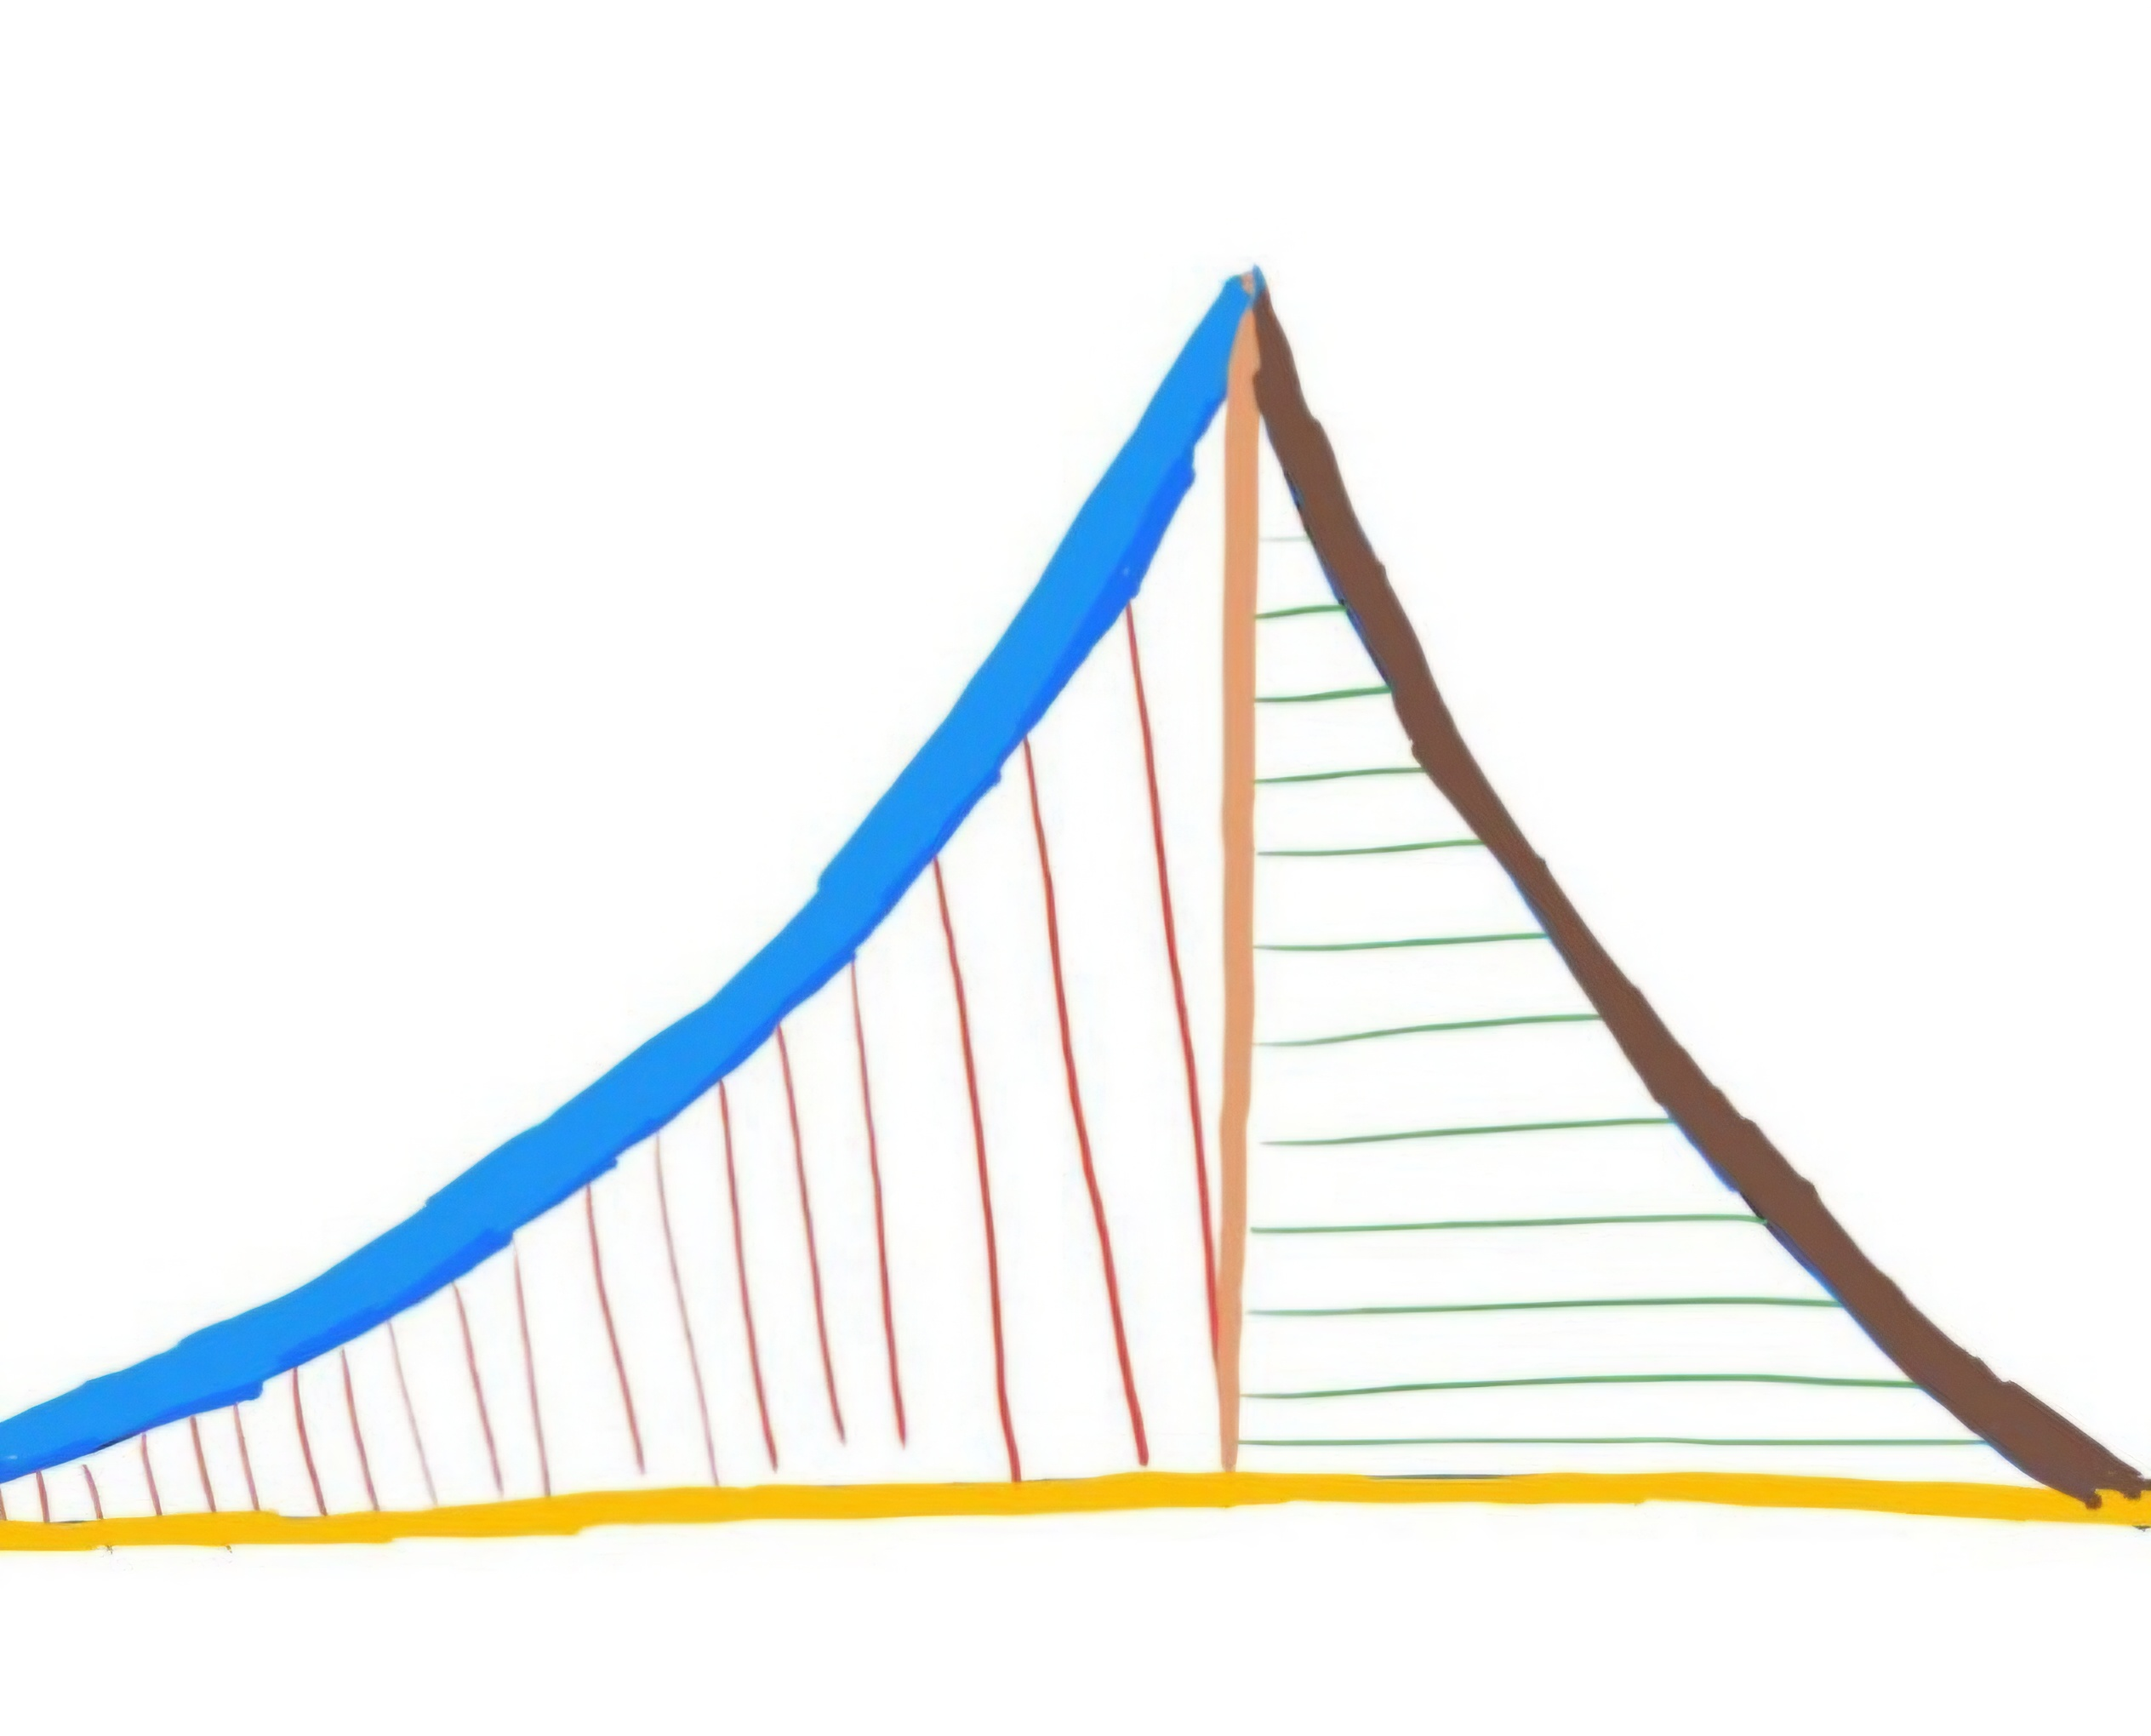
\includegraphics[width=0.2\columnwidth]{figs/logo.jpg}
        \\
        {\huge G. V. V. Sharma}
    \end{center}
}
\maketitle

\newpage
\section*{About this Book}

This book introduces matrices through high school coordinate geometry.
This approach makes it easier for beginners to learn Python for scientific
computing. All problems in the book are from NCERT mathematics textbooks
from Class 9--12. Exercises are from CBSE board exam papers.

The content is sufficient for industry jobs and covers nearly all matrix
prerequisites for machine learning. There is no copyright, so readers are
free to print and share.
License: https://creativecommons.org/licenses/by-sa/3.0/
\\
and
\\
https://www.gnu.org/licenses/fdl-1.3.en.html
\\
First manual appeared in January 2018
\\
First edition published on July 10, 2024
\\
In this edition, some incorrect solutions were removed. All figures
redrawn. More problems added.

\newpage
\onecolumn
\begin{center}
{\Large\bfseries CBSE 2026 10th class maths solutions (65-4-1)}
\end{center}
\vspace{0.4em}

\begin{list}{}{\setlength{\leftmargin}{1.15cm}\setlength{\labelwidth}{1.0cm}\setlength{\labelsep}{0.15cm}\setlength{\itemindent}{0pt}\setlength{\listparindent}{0pt}\setlength{\parsep}{0pt}\setlength{\topsep}{0pt}}
\item[4.1.4] If $PQ$ and $PR$ are tangents to the circle with centre $O$ and radius $4$ cm such that $\angle QPR=90^\circ$, find the length $OP$.

\begin{enumerate}
    \item[(A)] $4$ cm
    \item[(B)] $4\sqrt{2}$ cm
    \item[(C)] $8$ cm
    \item[(D)] $2\sqrt{2}$ cm
\end{enumerate}

\vspace{0.7em}\par\noindent\textbf{Solution:}

The radii to the points of contact are perpendicular to the tangents, so $\angle OQP=90^\circ$ and $\angle ORP=90^\circ$. The right triangles $\triangle OPQ$ and $\triangle OPR$ are congruent, so $OP$ bisects $\angle QPR$. Hence $\angle QPO=45^\circ$. In right triangle $OPQ$,
\[
\sin 45^\circ=\frac{OQ}{OP}=\frac{4}{OP},
\qquad OP=4\sqrt{2}\text{ cm}.
\]
Therefore, the correct answer is \textbf{(B)}.

The following code draws the tangent configuration and calculates $OP$.
\begin{lstlisting}[frame=single, basicstyle=\rmfamily, escapeinside={(*@}{@*)}]
(*@\makebox[\dimexpr\linewidth-2\fboxsep-2\fboxrule\relax][c]{codes/4.1.4.py}@*)
\end{lstlisting}
\begin{figure}[H]
    \centering
    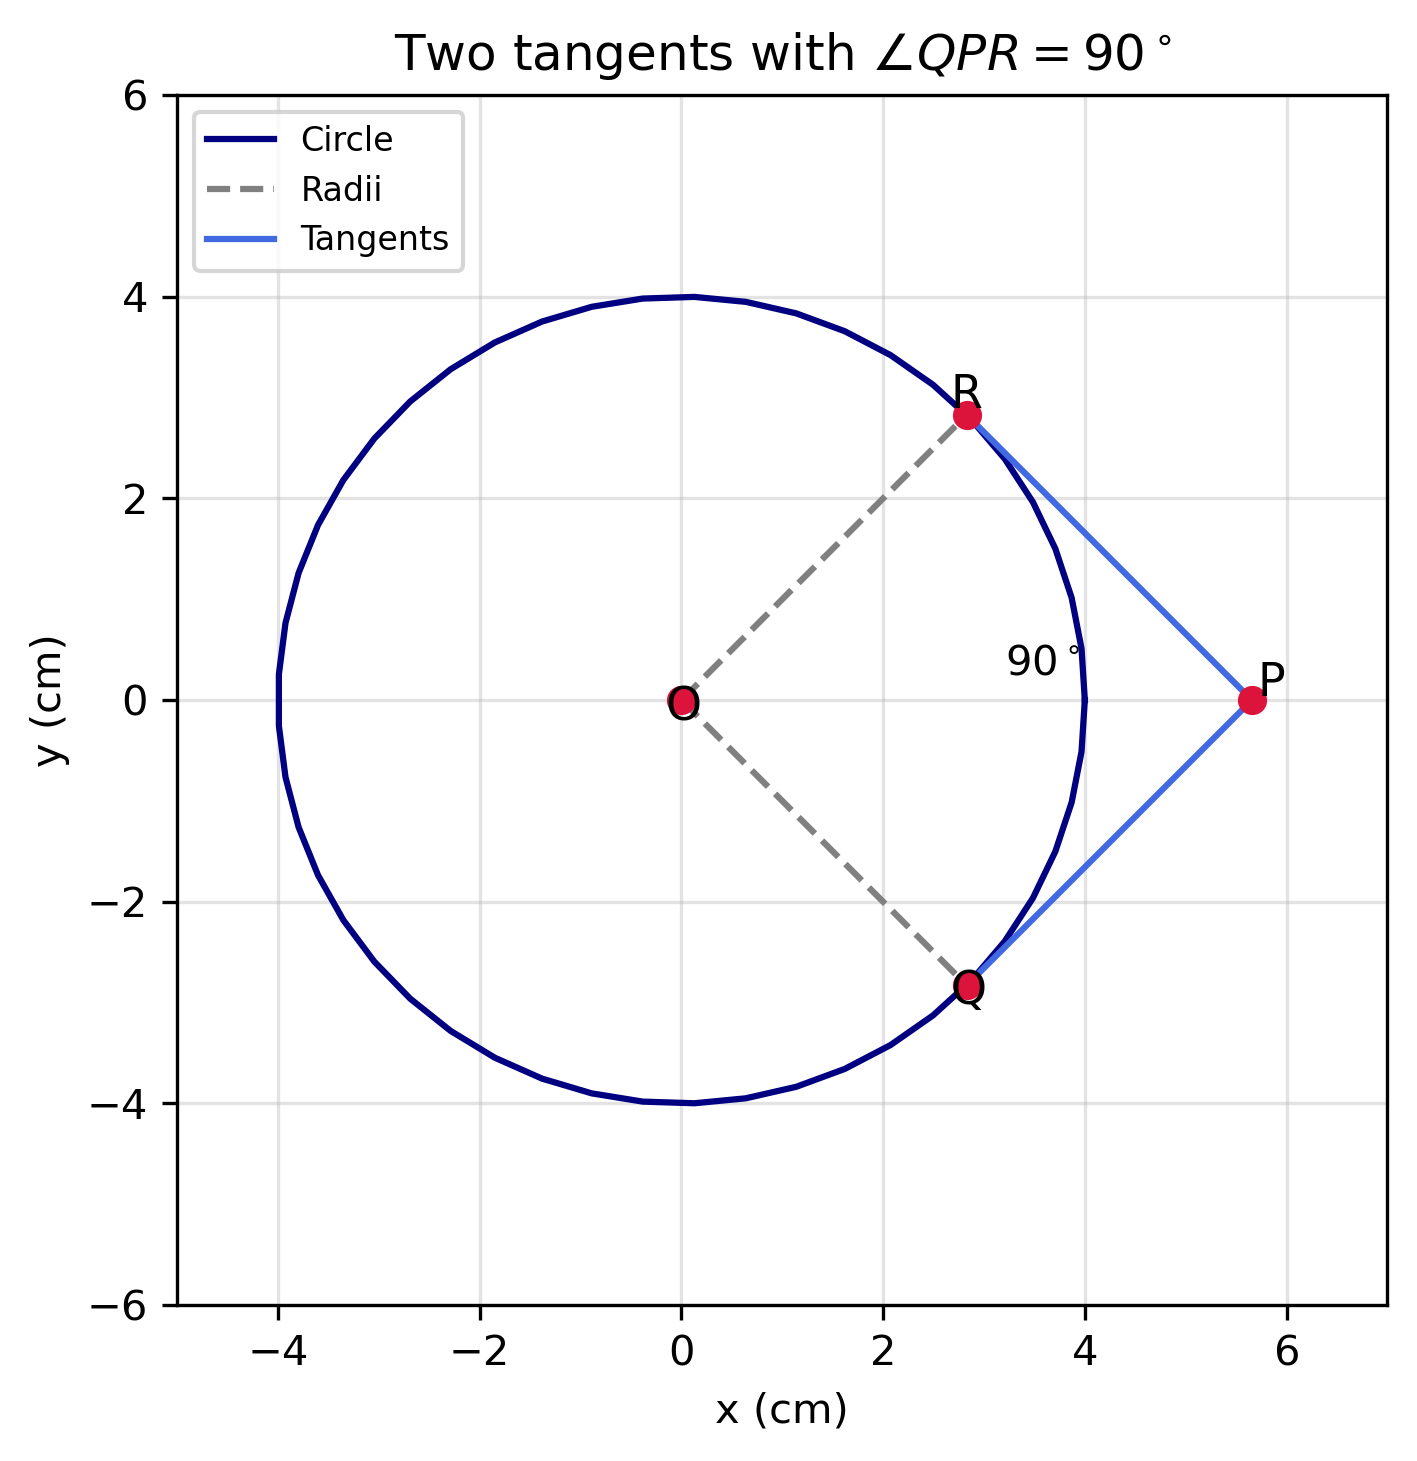
\includegraphics[width=0.62\linewidth]{figs/4.1.4.png}
    \caption{Tangents $PQ$ and $PR$ to a circle of radius $4$ cm, with $\angle QPR=90^\circ$.}
    \label{fig:4.1.4}
\end{figure}
\end{list}

\newpage
\begin{list}{}{\setlength{\leftmargin}{1.15cm}\setlength{\labelwidth}{1.0cm}\setlength{\labelsep}{0.15cm}\setlength{\itemindent}{0pt}\setlength{\listparindent}{0pt}\setlength{\parsep}{0pt}\setlength{\topsep}{0pt}}
\item[4.1.7] In the given figure, a circle is centred at $(1,2)$. Find the diameter of the circle.

\begin{enumerate}
    \item[(A)] $4$
    \item[(B)] $2\sqrt{2}$
    \item[(C)] $\sqrt{5}$
    \item[(D)] $2\sqrt{5}$
\end{enumerate}

\vspace{0.7em}\par\noindent\textbf{Solution:}

From the figure, the endpoints of the diameter are $(0,4)$ and $(2,0)$. Their midpoint is $(1,2)$, the given centre. Hence the diameter is
\[
\sqrt{(2-0)^2+(0-4)^2}=\sqrt{4+16}=2\sqrt{5}.
\]
The correct answer is \textbf{(D)}.

The following code plots the circle and diameter, then calculates the diameter.
\begin{lstlisting}[frame=single, basicstyle=\rmfamily, escapeinside={(*@}{@*)}]
(*@\makebox[\dimexpr\linewidth-2\fboxsep-2\fboxrule\relax][c]{codes/4.1.7.py}@*)
\end{lstlisting}
\begin{figure}[H]
    \centering
    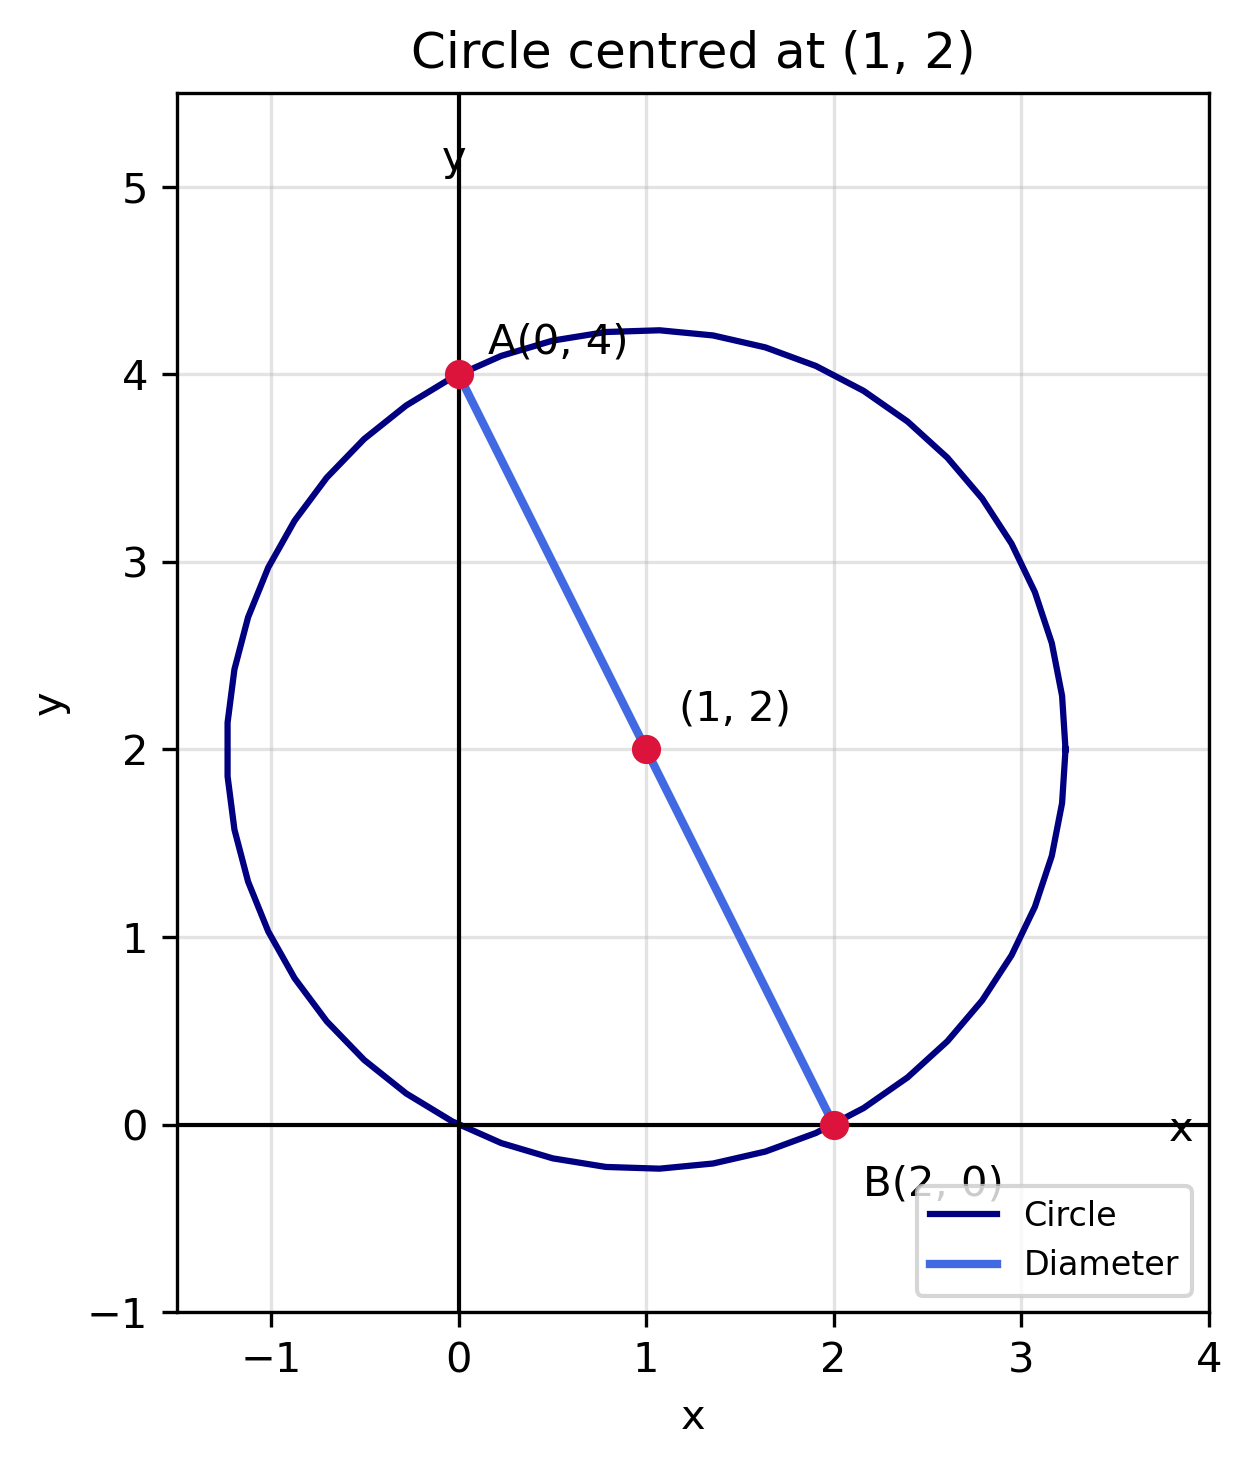
\includegraphics[width=0.56\linewidth]{figs/4.1.7.png}
    \caption{Circle centred at $(1,2)$ with the diameter endpoints shown.}
    \label{fig:4.1.7}
\end{figure}
\end{list}


\newpage
\begin{list}{}{\setlength{\leftmargin}{1.15cm}\setlength{\labelwidth}{1.0cm}\setlength{\labelsep}{0.15cm}\setlength{\itemindent}{0pt}\setlength{\listparindent}{0pt}\setlength{\parsep}{0pt}\setlength{\topsep}{0pt}}
\item[4.1.8] The value of $k$ for which the system of linear equations $\dfrac{x}{2}+\dfrac{y}{3}=5$ and $2x+ky=7$ is inconsistent, is:

\begin{enumerate}
    \item[(A)] $\dfrac{3}{4}$
    \item[(B)] $\dfrac{4}{3}$
    \item[(C)] $\dfrac{1}{3}$
    \item[(D)] $3$
\end{enumerate}

\vspace{0.7em}\par\noindent\textbf{Solution:}

The first equation is $3x+2y=30$. For the two lines to be parallel, $\dfrac{3}{2}=\dfrac{2}{k}$, so $k=\dfrac{4}{3}$. Their constant terms are not in the same ratio, so the lines are distinct and the system is inconsistent. The correct answer is \textbf{(B)}.

The following code plots the two parallel lines.
\begin{lstlisting}[frame=single, basicstyle=\rmfamily, escapeinside={(*@}{@*)}]
(*@\makebox[\dimexpr\linewidth-2\fboxsep-2\fboxrule\relax][c]{codes/4.1.8.py}@*)
\end{lstlisting}
\begin{figure}[H]
    \centering
    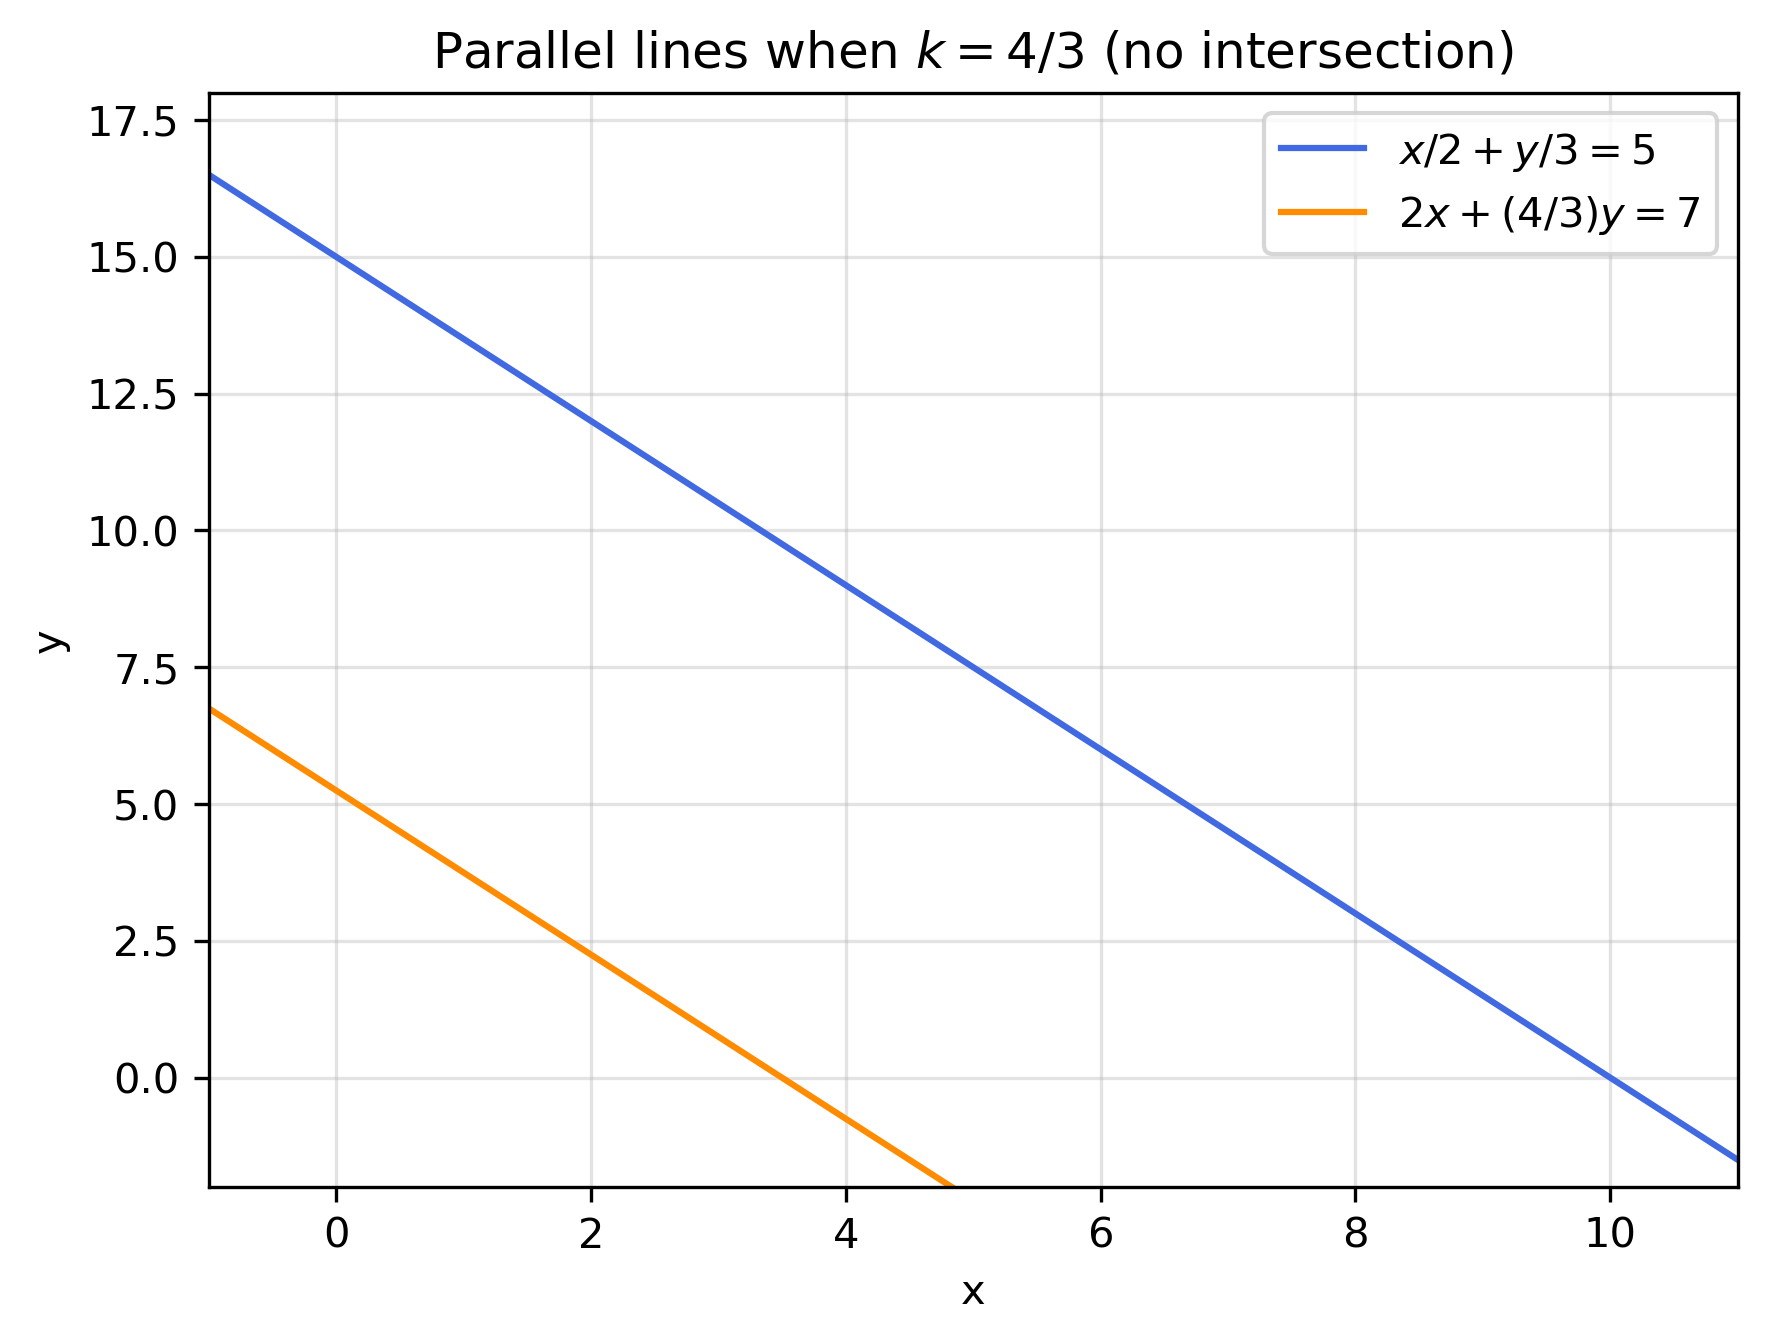
\includegraphics[width=0.58\linewidth]{figs/4.1.8.png}
    \caption{The parallel lines for $k=\dfrac{4}{3}$; they have no point of intersection.}
    \label{fig:4.1.8}
\end{figure}
\end{list}

\vspace{1.2em}
\newpage
\begin{list}{}{\setlength{\leftmargin}{1.15cm}\setlength{\labelwidth}{1.0cm}\setlength{\labelsep}{0.15cm}\setlength{\itemindent}{0pt}\setlength{\listparindent}{0pt}\setlength{\parsep}{0pt}\setlength{\topsep}{0pt}}
\item[4.1.10] Two different dice are rolled together. Find the probability that both obtained numbers are less than $4$.

\begin{enumerate}
    \item[(A)] $\dfrac{2}{9}$
    \item[(B)] $\dfrac{7}{36}$
    \item[(C)] $\dfrac{1}{4}$
    \item[(D)] $\dfrac{2}{3}$
\end{enumerate}

\vspace{0.7em}\par\noindent\textbf{Solution:}

Each die can show $1$, $2$, or $3$, giving $3\times3=9$ favourable outcomes out of $36$ equally likely outcomes. Thus, $P=\dfrac{9}{36}=\dfrac{1}{4}$. The correct answer is \textbf{(C)}. The code simulates $500{,}000$ rolls and plots the empirical and theoretical probability distributions for the event.

\begin{lstlisting}[frame=single, basicstyle=\rmfamily, escapeinside={(*@}{@*)}]
(*@\makebox[\dimexpr\linewidth-2\fboxsep-2\fboxrule\relax][c]{codes/4.1.10.py}@*)
\end{lstlisting}
\begin{figure}[H]
    \centering
    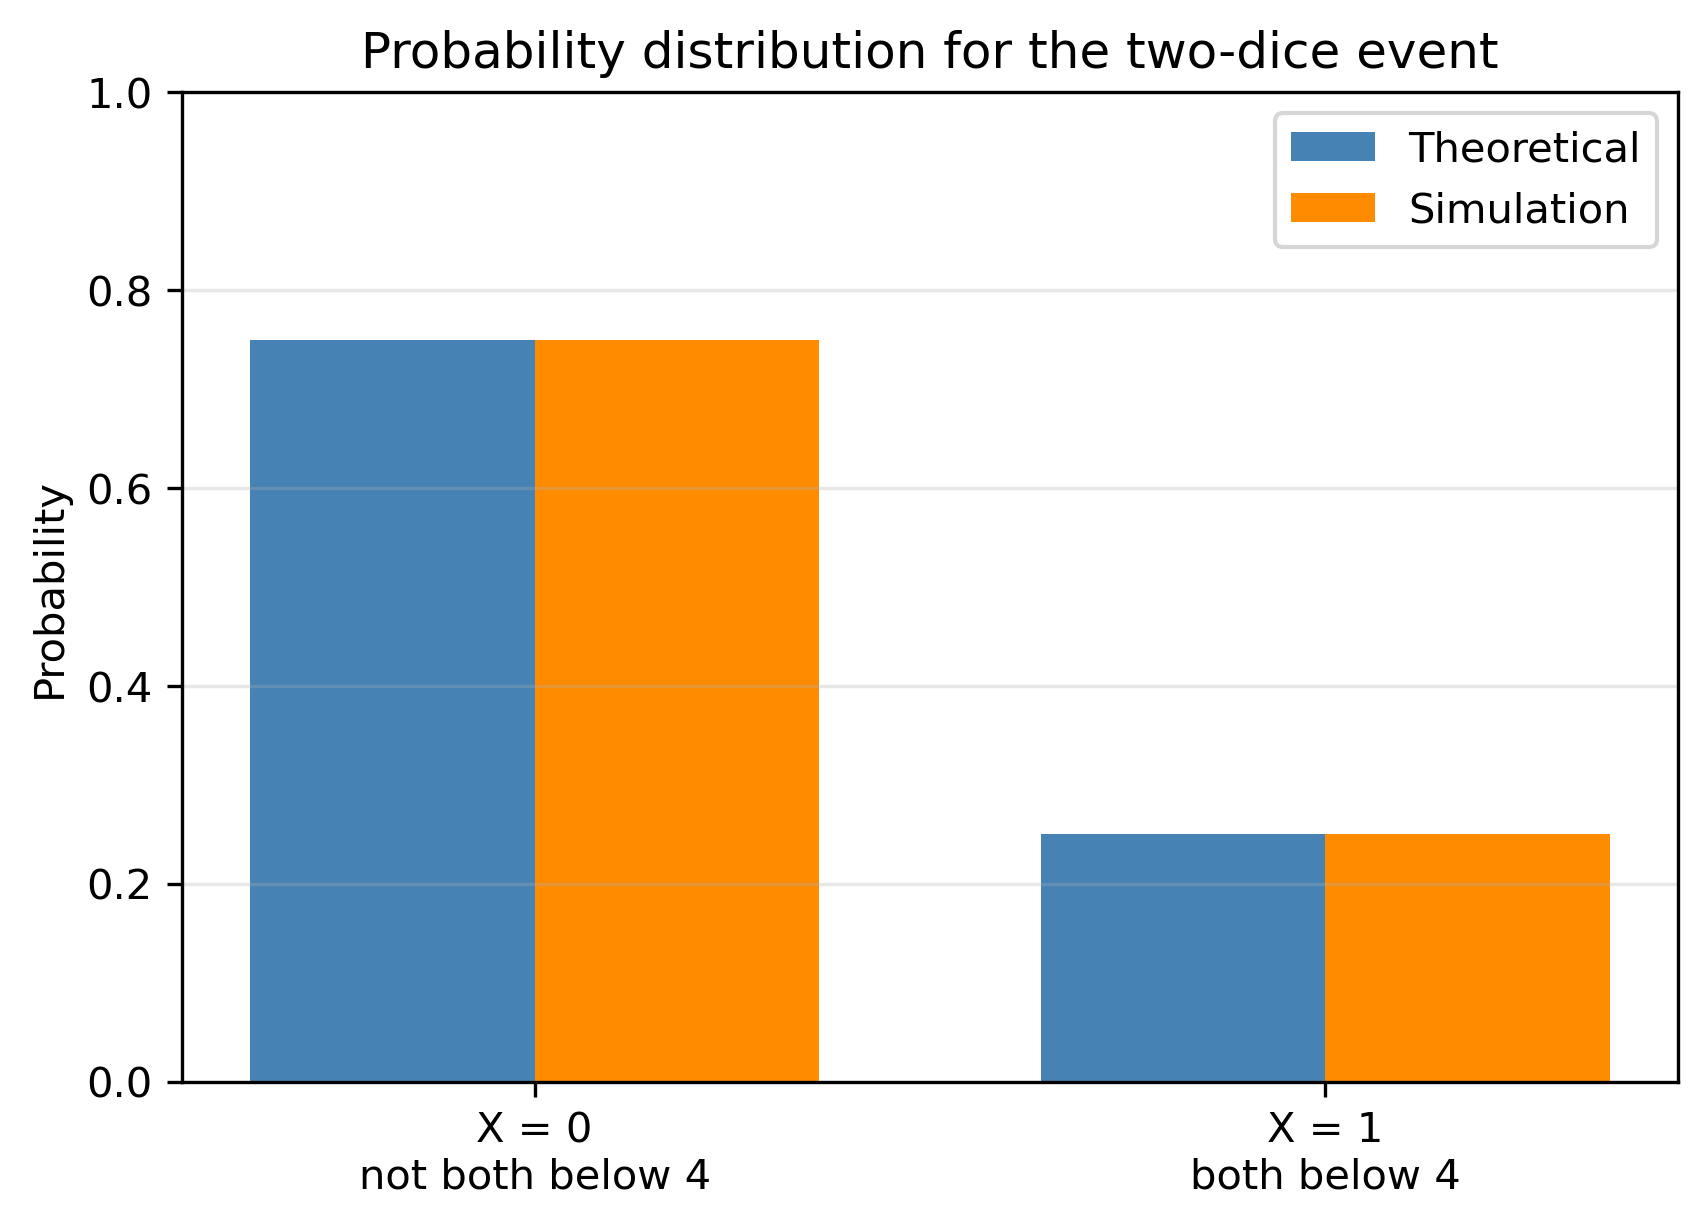
\includegraphics[width=0.56\linewidth]{figs/4.1.10.png}
    \caption{Probability distribution of $X$, where $X=1$ if both dice show a number below $4$, and $X=0$ otherwise.}
    \label{fig:4.1.10}
\end{figure}
\end{list}

\vspace{1.2em}
\newpage
\begin{list}{}{\setlength{\leftmargin}{1.15cm}\setlength{\labelwidth}{1.0cm}\setlength{\labelsep}{0.15cm}\setlength{\itemindent}{0pt}\setlength{\listparindent}{0pt}\setlength{\parsep}{0pt}\setlength{\topsep}{0pt}}
\item[4.1.14] $PQ$ is tangent to a circle with centre $O$. If $\angle POR=65^\circ$, find $m\angle PTR$.

\begin{enumerate}
    \item[(A)] $65^\circ$
    \item[(B)] $58.5^\circ$
    \item[(C)] $57.5^\circ$
    \item[(D)] $45^\circ$
\end{enumerate}

\vspace{0.7em}\par\noindent\textbf{Solution:}

Since $OP$ is a radius to the point of tangency, $OP\perp PQ$, so $\angle SPT=90^\circ$. The inscribed angle $\angle PSR$ subtending arc $PR$ is half the central angle $\angle POR$, hence $\angle PST=\angle PSR=32.5^\circ$ because $S$, $R$, and $T$ are collinear. Therefore, in $\triangle PST$,
\[
\angle PTR=\angle PTS=180^\circ-90^\circ-32.5^\circ=57.5^\circ.
\]
The correct answer is \textbf{(C)}.

The following code draws the circle, tangent and secant, and calculates $\angle PTR$.
\begin{lstlisting}[frame=single, basicstyle=\rmfamily, escapeinside={(*@}{@*)}]
(*@\makebox[\dimexpr\linewidth-2\fboxsep-2\fboxrule\relax][c]{codes/4.1.14.py}@*)
\end{lstlisting}
\begin{figure}[H]
    \centering
    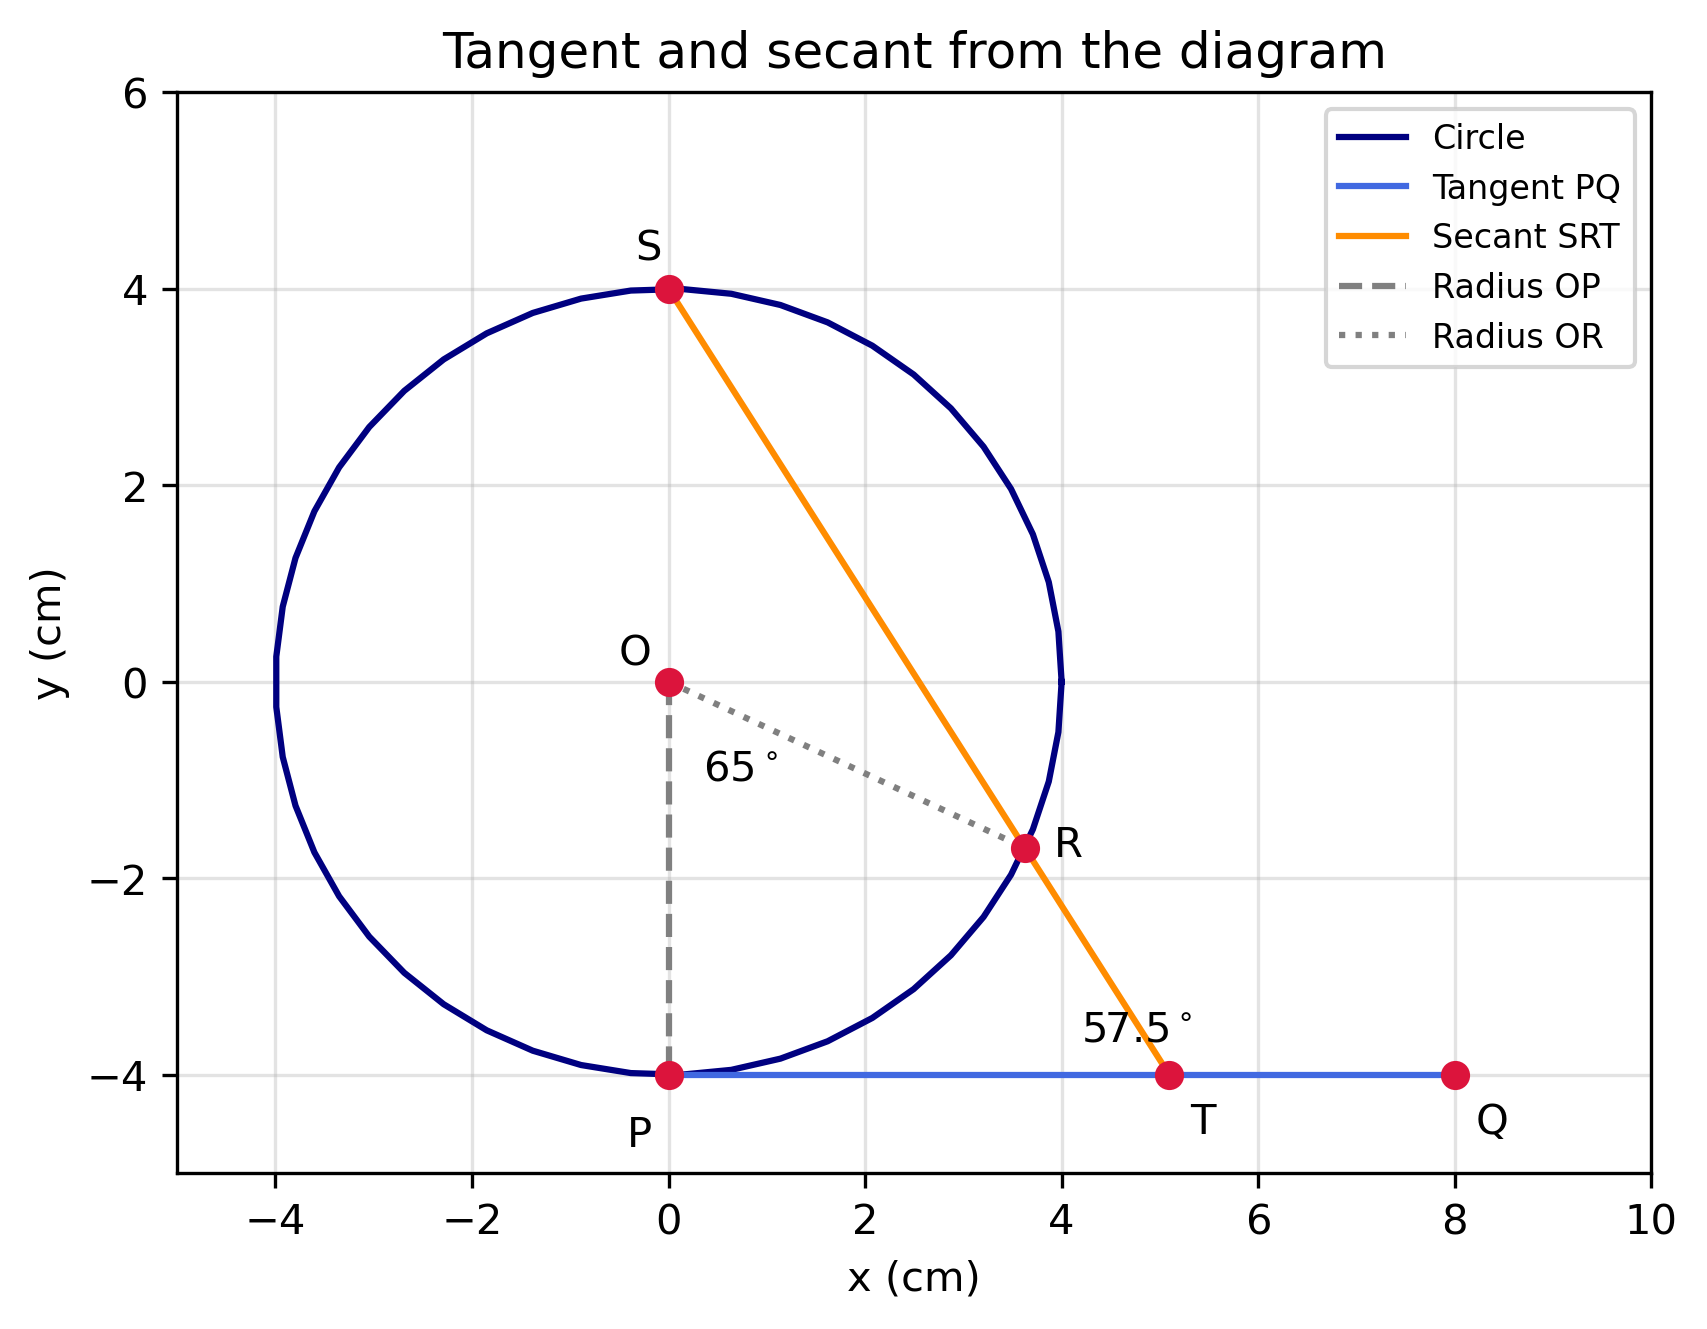
\includegraphics[width=0.58\linewidth]{figs/4.1.14.png}
    \caption{Tangent $PQ$ and secant $SRT$ with central angle $\angle POR=65^\circ$.}
    \label{fig:4.1.14}
\end{figure}
\end{list}

\newpage
\begin{list}{}{\setlength{\leftmargin}{1.15cm}\setlength{\labelwidth}{1.0cm}\setlength{\labelsep}{0.15cm}\setlength{\itemindent}{0pt}\setlength{\listparindent}{0pt}\setlength{\parsep}{0pt}\setlength{\topsep}{0pt}}
\item[4.1.17] Arc $PQ$ subtends an angle $\theta$ at the centre of a circle of radius $6.3$ cm. If the length of arc $PQ$ is $11$ cm, find $\theta$.

\noindent (A) $10^\circ$ \hfill (B) $60^\circ$ \hfill (C) $45^\circ$ \hfill (D) $100^\circ$

\vspace{0.7em}\par\noindent\textbf{Solution:}

Using arc length $s=r\theta$ (with $\theta$ in radians),
\[
\theta=\frac{11}{6.3}\text{ radians}=100^\circ.
\]
The correct answer is \textbf{(D)}.

The code draws the arc and radii, and calculates the angle.
\begin{lstlisting}[frame=single, basicstyle=\rmfamily, escapeinside={(*@}{@*)}]
(*@\makebox[\dimexpr\linewidth-2\fboxsep-2\fboxrule\relax][c]{codes/4.1.17.py}@*)
\end{lstlisting}
\begin{figure}[H]
    \centering
    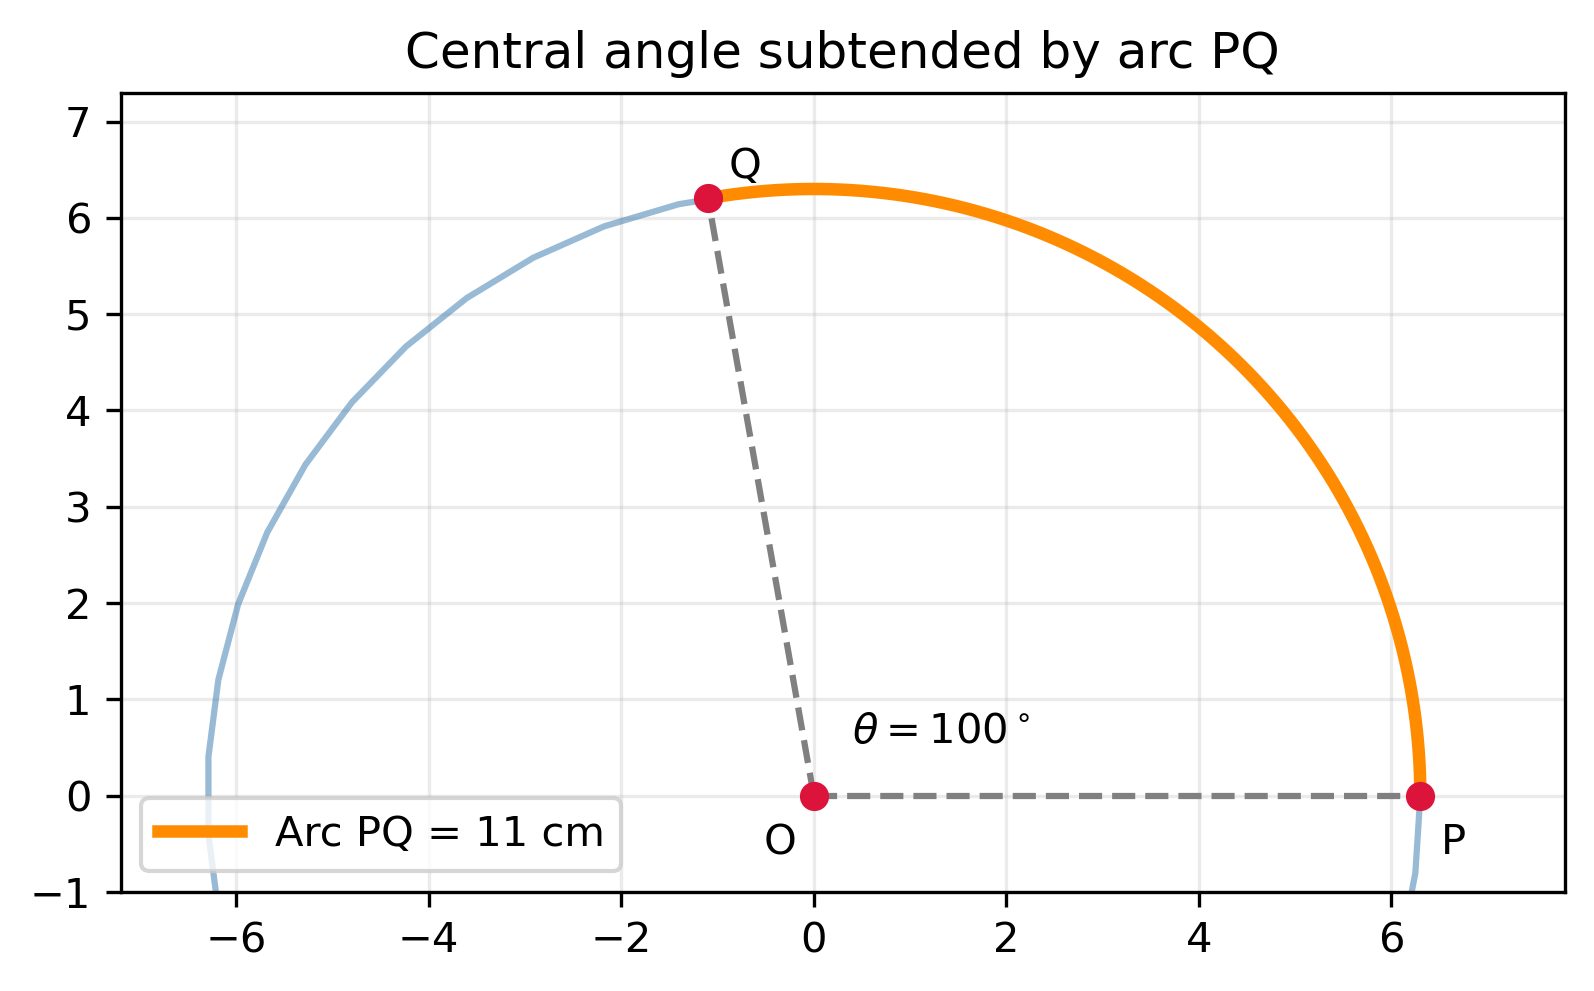
\includegraphics[width=0.53\linewidth]{figs/4.1.17.png}
    \caption{Arc $PQ$ of length $11$ cm subtending $100^\circ$ at the centre.}
\end{figure}
\end{list}

\vspace{1.2em}
\begin{list}{}{\setlength{\leftmargin}{1.15cm}\setlength{\labelwidth}{1.0cm}\setlength{\labelsep}{0.15cm}\setlength{\itemindent}{0pt}\setlength{\listparindent}{0pt}\setlength{\parsep}{0pt}\setlength{\topsep}{0pt}}
\item[4.1.21] Verify that the roots of $(p-q)x^2+(q-r)x+(r-p)=0$ are equal when $q+r=2p$.

\vspace{0.7em}\par\noindent\textbf{Solution:}

Put $r=2p-q$. Then the equation becomes
\[
(p-q)x^2+2(q-p)x+(p-q)=0
\quad\Longrightarrow\quad
(p-q)(x-1)^2=0.
\]
Thus both roots are $x=1$ (for the non-degenerate quadratic case), so the roots are equal.
\end{list}

\vspace{1.2em}
\begin{list}{}{\setlength{\leftmargin}{1.15cm}\setlength{\labelwidth}{1.0cm}\setlength{\labelsep}{0.15cm}\setlength{\itemindent}{0pt}\setlength{\listparindent}{0pt}\setlength{\parsep}{0pt}\setlength{\topsep}{0pt}}
\item[4.1.22] $D$ is a point on side $BC$ of $\triangle ABC$ such that $\angle CAB=\angle CDA$. Show that $CA^2=CB\times CD$.

\vspace{0.7em}\par\noindent\textbf{Solution:}

Since $D$ lies on $BC$, $\angle ACB=\angle DCA$. With the given $\angle CAB=\angle CDA$, $\triangle CAB\sim\triangle CDA$ (AA). Corresponding sides give
\[
\frac{CA}{CD}=\frac{CB}{CA},
\qquad\therefore\qquad CA^2=CB\times CD.
\]

The following code draws a configuration satisfying the given angles and verifies the proportionality numerically.
\begin{lstlisting}[frame=single, basicstyle=\rmfamily, escapeinside={(*@}{@*)}]
(*@\makebox[\dimexpr\linewidth-2\fboxsep-2\fboxrule\relax][c]{codes/4.1.22.py}@*)
\end{lstlisting}
\begin{figure}[H]
    \centering
    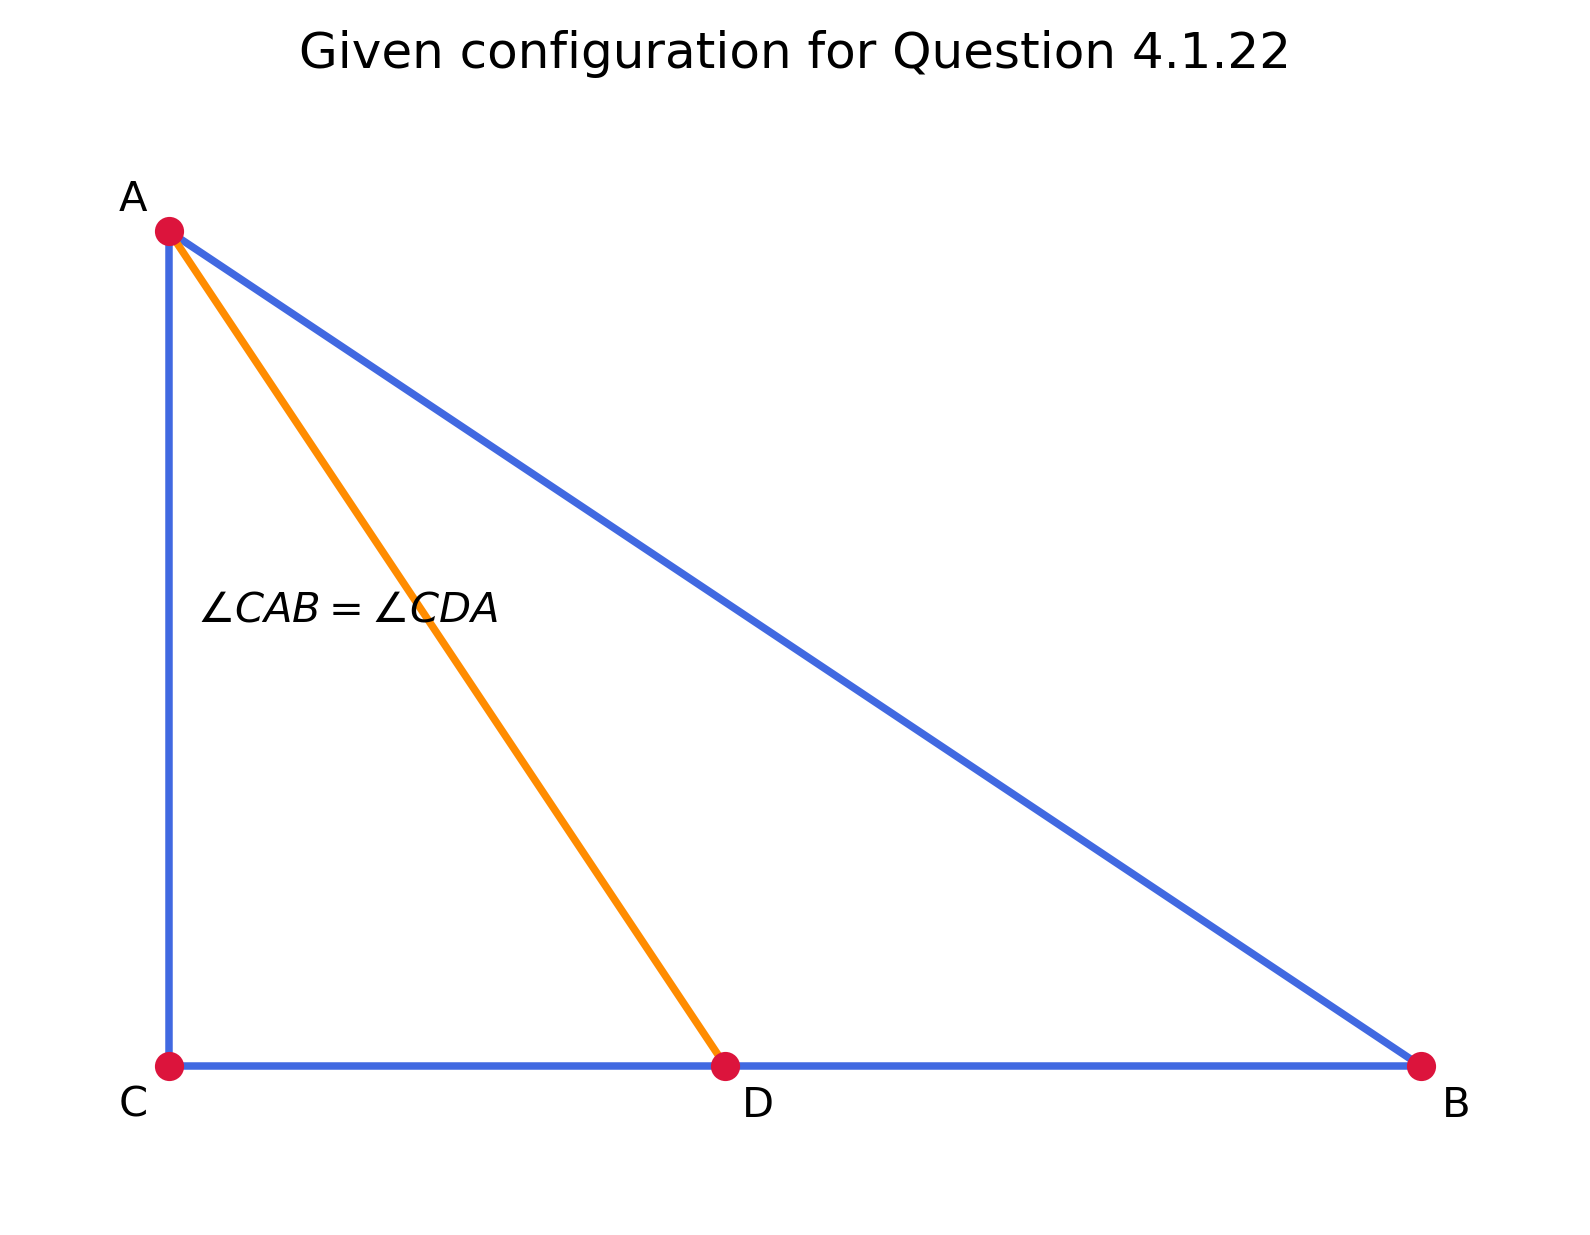
\includegraphics[width=0.50\linewidth]{figs/4.1.22.png}
    \caption{Triangle $ABC$ with $D$ on $BC$ and $AD$ drawn.}
\end{figure}
\end{list}

\vspace{1.2em}
\begin{list}{}{\setlength{\leftmargin}{1.15cm}\setlength{\labelwidth}{1.0cm}\setlength{\labelsep}{0.15cm}\setlength{\itemindent}{0pt}\setlength{\listparindent}{0pt}\setlength{\parsep}{0pt}\setlength{\topsep}{0pt}}
\item[4.1.26.1] In a class test, Veer scored 6 more than twice Kevin's marks. If one of them had scored 4 more marks, their total would have been 40. Find Veer's and Kevin's marks.

\vspace{0.7em}\par\noindent\textbf{Solution:}

Let Kevin's marks be $K$ and Veer's be $V$. Then $V=2K+6$ and $V+K+4=40$, so $3K+10=40$. Thus $K=10$ and $V=26$ marks.

The code plots the two relationships and marks their intersection.
\begin{lstlisting}[frame=single, basicstyle=\rmfamily, escapeinside={(*@}{@*)}]
(*@\makebox[\dimexpr\linewidth-2\fboxsep-2\fboxrule\relax][c]{codes/4.1.26.1.py}@*)
\end{lstlisting}
\begin{figure}[H]
    \centering
    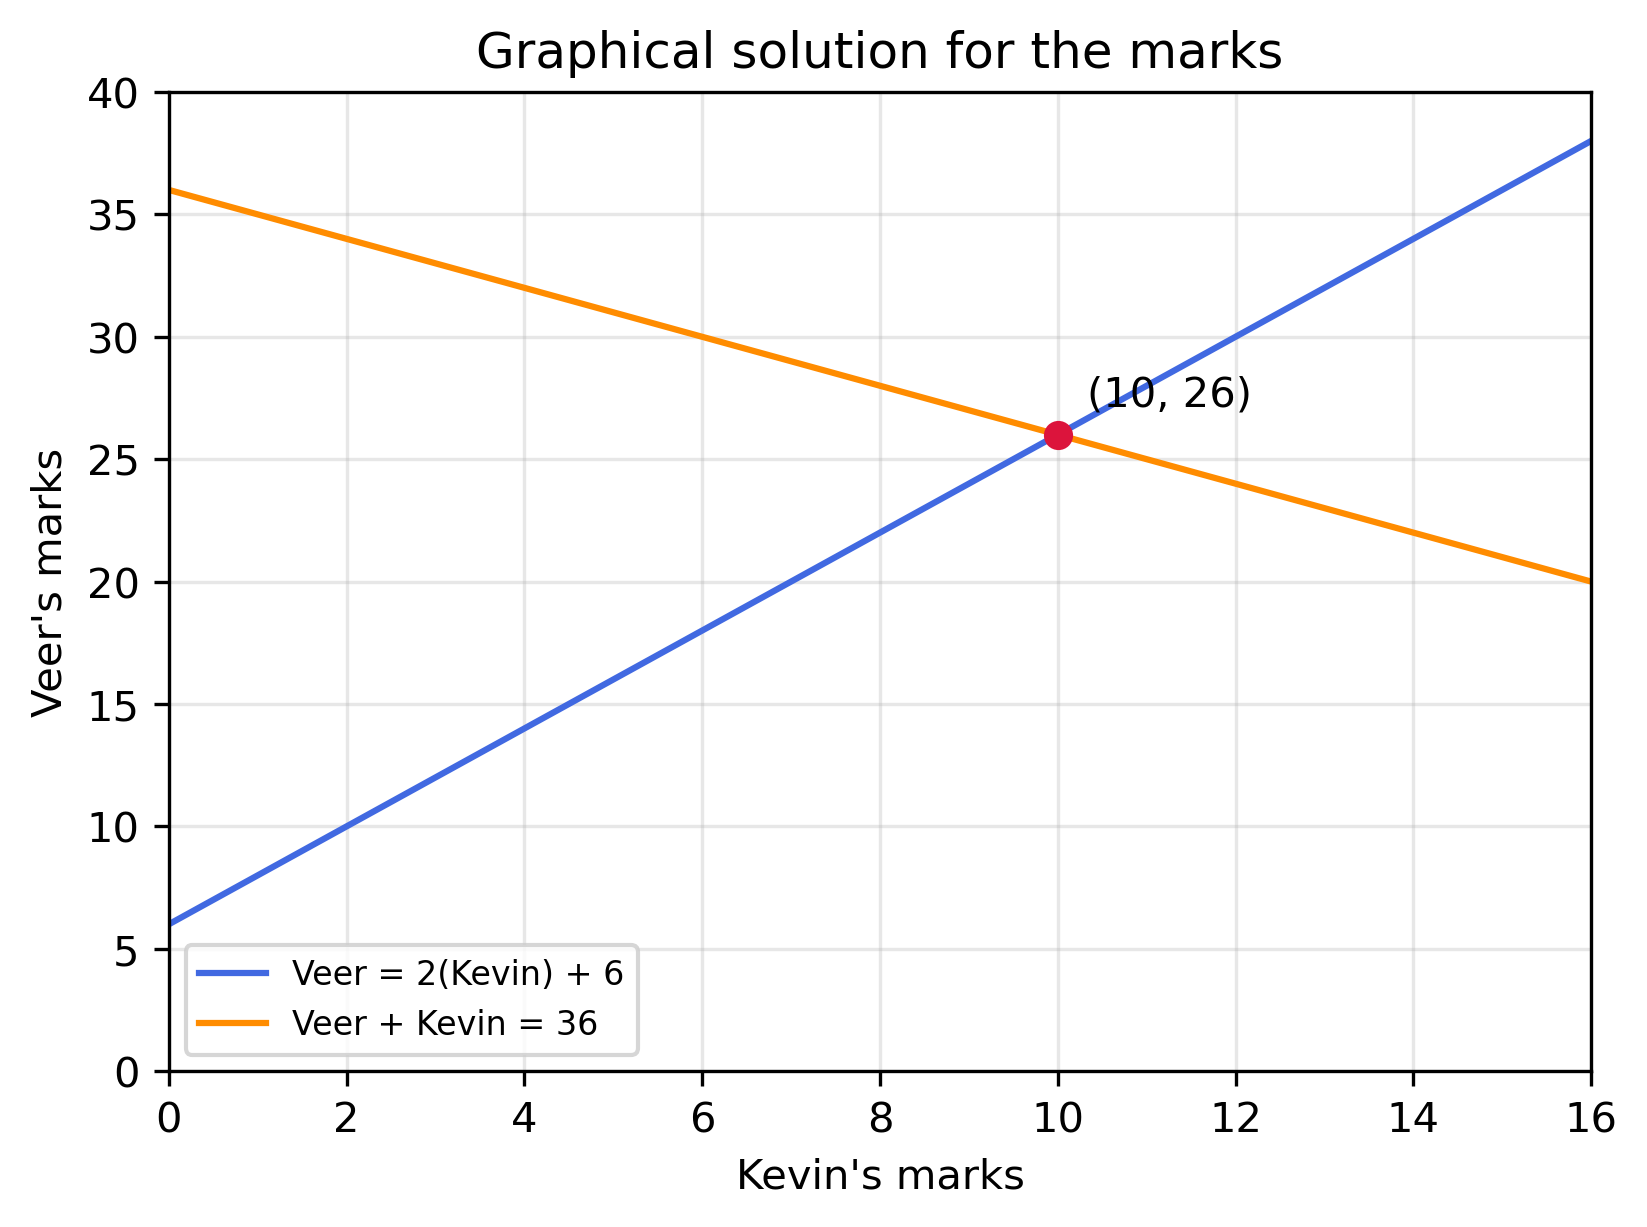
\includegraphics[width=0.50\linewidth]{figs/4.1.26.1.png}
    \caption{Veer and Kevin's marks at the intersection of the two lines.}
\end{figure}

\item[4.1.26.2] Solve the linear equations $3x+y=14$ and $y=2$ graphically.

\vspace{0.7em}\par\noindent\textbf{Solution:}

The lines $y=14-3x$ and $y=2$ intersect at $(4,2)$. Hence the solution is $\boxed{x=4,\ y=2}$.

The code plots both lines and marks their intersection.
\begin{lstlisting}[frame=single, basicstyle=\rmfamily, escapeinside={(*@}{@*)}]
(*@\makebox[\dimexpr\linewidth-2\fboxsep-2\fboxrule\relax][c]{codes/4.1.26.2.py}@*)
\end{lstlisting}
\begin{figure}[H]
    \centering
    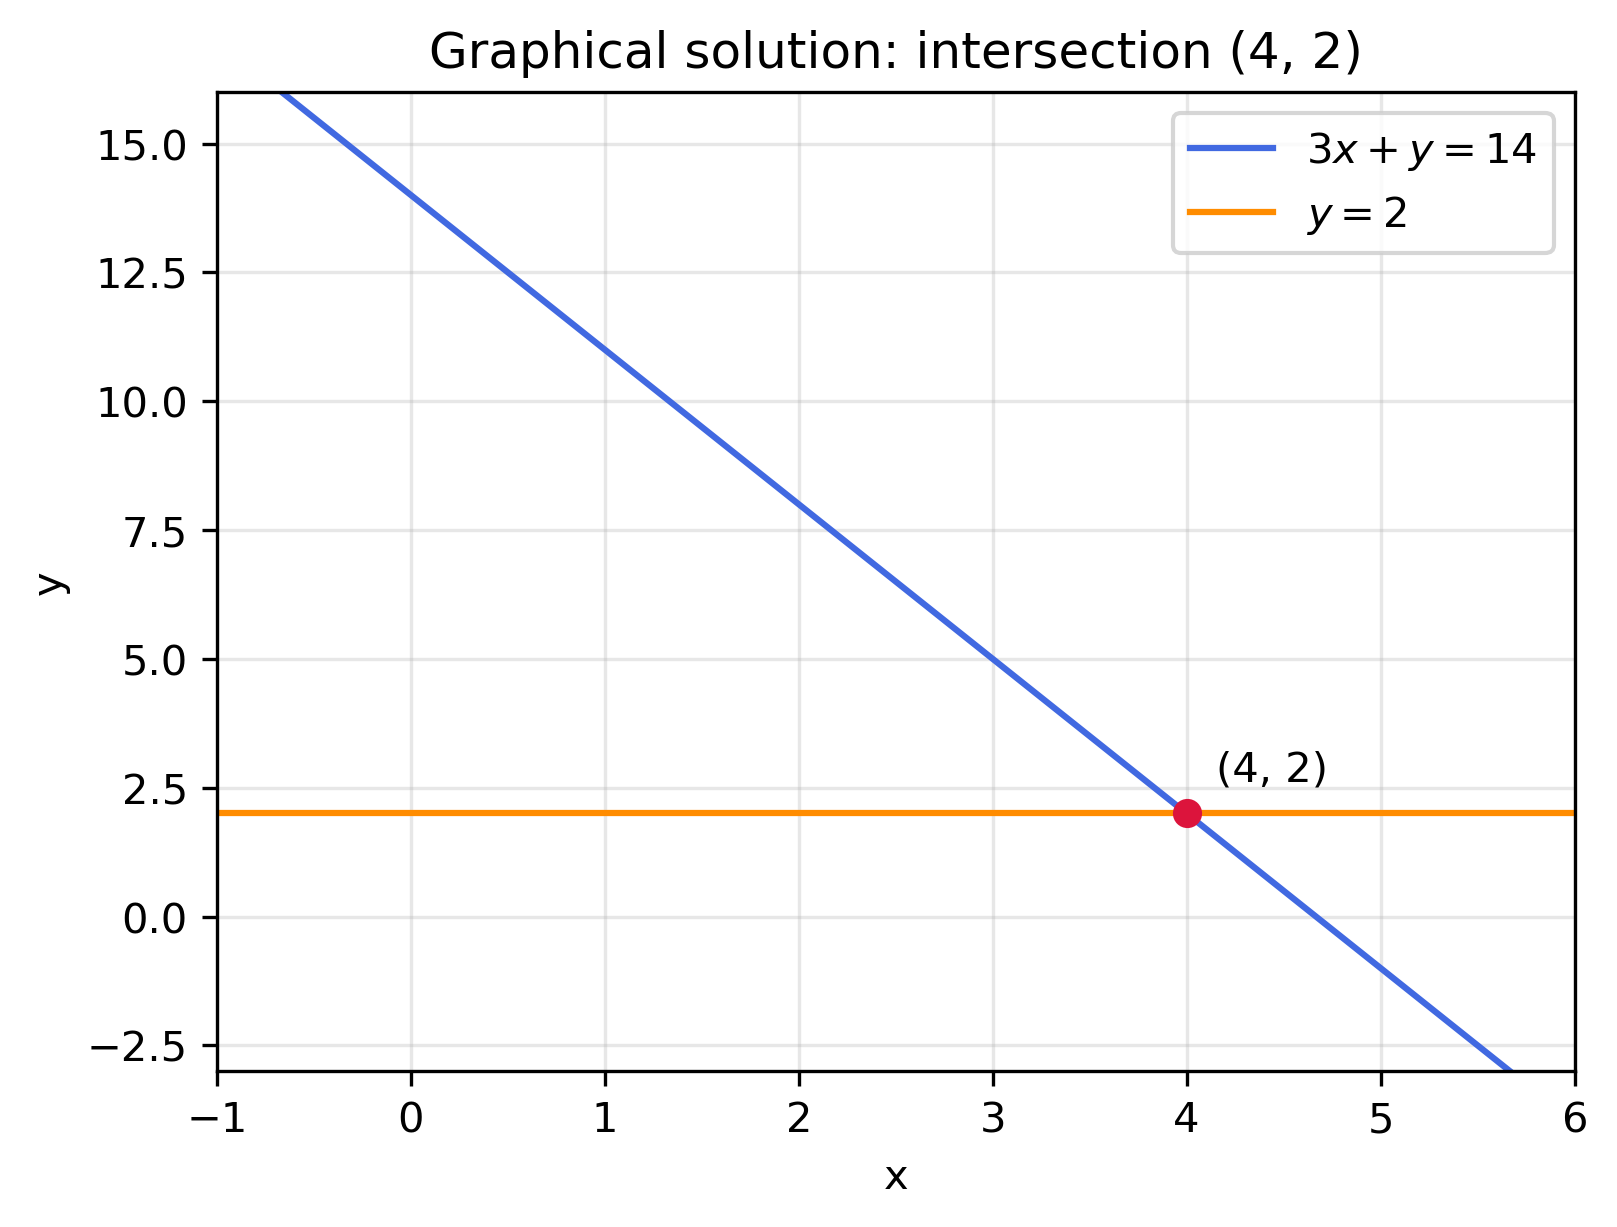
\includegraphics[width=0.52\linewidth]{figs/4.1.26.2.png}
    \caption{Graphical solution of the pair of linear equations.}
\end{figure}
\end{list}

\newpage
\begin{list}{}{\setlength{\leftmargin}{1.15cm}\setlength{\labelwidth}{1.0cm}\setlength{\labelsep}{0.15cm}\setlength{\itemindent}{0pt}\setlength{\listparindent}{0pt}\setlength{\parsep}{0pt}\setlength{\topsep}{0pt}}
\item[4.1.30] A bag contains 30 balls, of which $m$ are blue. (i) Find the probability that a ball drawn at random is not blue. (ii) If 6 more blue balls are added, the probability of drawing a blue ball becomes $\frac54$ times its original value. Find $m$.

\vspace{0.7em}\par\noindent\textbf{Solution:}

(i) The number of non-blue balls is $30-m$, so $P(\text{not blue})=\dfrac{30-m}{30}$.\\
(ii) The new probability is $\dfrac{m+6}{36}$. Therefore
\[
\frac{m+6}{36}=\frac54\cdot\frac{m}{30}
\quad\Longrightarrow\quad m=12.
\]
There are $12$ blue balls initially.
\end{list}

\vspace{1.2em}
\begin{list}{}{\setlength{\leftmargin}{1.15cm}\setlength{\labelwidth}{1.0cm}\setlength{\labelsep}{0.15cm}\setlength{\itemindent}{0pt}\setlength{\listparindent}{0pt}\setlength{\parsep}{0pt}\setlength{\topsep}{0pt}}
\item[4.1.31] Find the greatest number less than $10{,}000$ that is exactly divisible by $48$, $60$, and $65$.

\vspace{0.7em}\par\noindent\textbf{Solution:}

\[
\operatorname{LCM}(48,60,65)=2^4\cdot3\cdot5\cdot13=3120.
\]
The greatest multiple of $3120$ below $10{,}000$ is $3\times3120=\boxed{9360}$.

The following C program calculates the LCM and the required greatest multiple.
\begin{lstlisting}[frame=single, basicstyle=\rmfamily, escapeinside={(*@}{@*)}]
(*@\makebox[\dimexpr\linewidth-2\fboxsep-2\fboxrule\relax][c]{codes/4.1.31.c}@*)
\end{lstlisting}
\end{list}

\vspace{0.3em}
\begin{list}{}{\setlength{\leftmargin}{1.15cm}\setlength{\labelwidth}{1.0cm}\setlength{\labelsep}{0.15cm}\setlength{\itemindent}{0pt}\setlength{\listparindent}{0pt}\setlength{\parsep}{0pt}\setlength{\topsep}{0pt}}
\item[4.1.33] In the figure, $TP$ and $TQ$ are tangents to the circle with centre $M$, touching the circle with centre $N$ at $A$ and $B$, respectively. Given $MQ=13$ cm, $NB=8$ cm, $BQ=35$ cm and $TP=80$ cm: (i) name quadrilateral $MQBN$; (ii) determine whether $MN\parallel PA$, with justification; (iii) find $TB$; (iv) find $MN$.

\vspace{0.7em}\par\noindent\textbf{Solution:}

(i) $MQ\parallel NB$ and both are perpendicular to $QB$, so $MQBN$ is a right trapezium.\\
(ii) No: the centres are $13$ cm and $8$ cm from tangent $PA$; hence $MN$ cannot be parallel to $PA$.\\
(iii) $TQ=TP=80$ cm and $TB=TQ-BQ$, so $TB=80-35=45$ cm.\\
(iv) The centres differ by $35$ cm parallel to $QB$ and by $13-8=5$ cm perpendicular to it. Thus $MN=\sqrt{35^2+5^2}=\boxed{25\sqrt2\text{ cm}}$.

The code draws the two-circle tangent configuration and prints the answers.
\begin{lstlisting}[frame=single, basicstyle=\rmfamily, escapeinside={(*@}{@*)}]
(*@\makebox[\dimexpr\linewidth-2\fboxsep-2\fboxrule\relax][c]{codes/4.1.33.py}@*)
\end{lstlisting}
\vspace{-0.6em}
\begin{figure}[H]
    \centering
    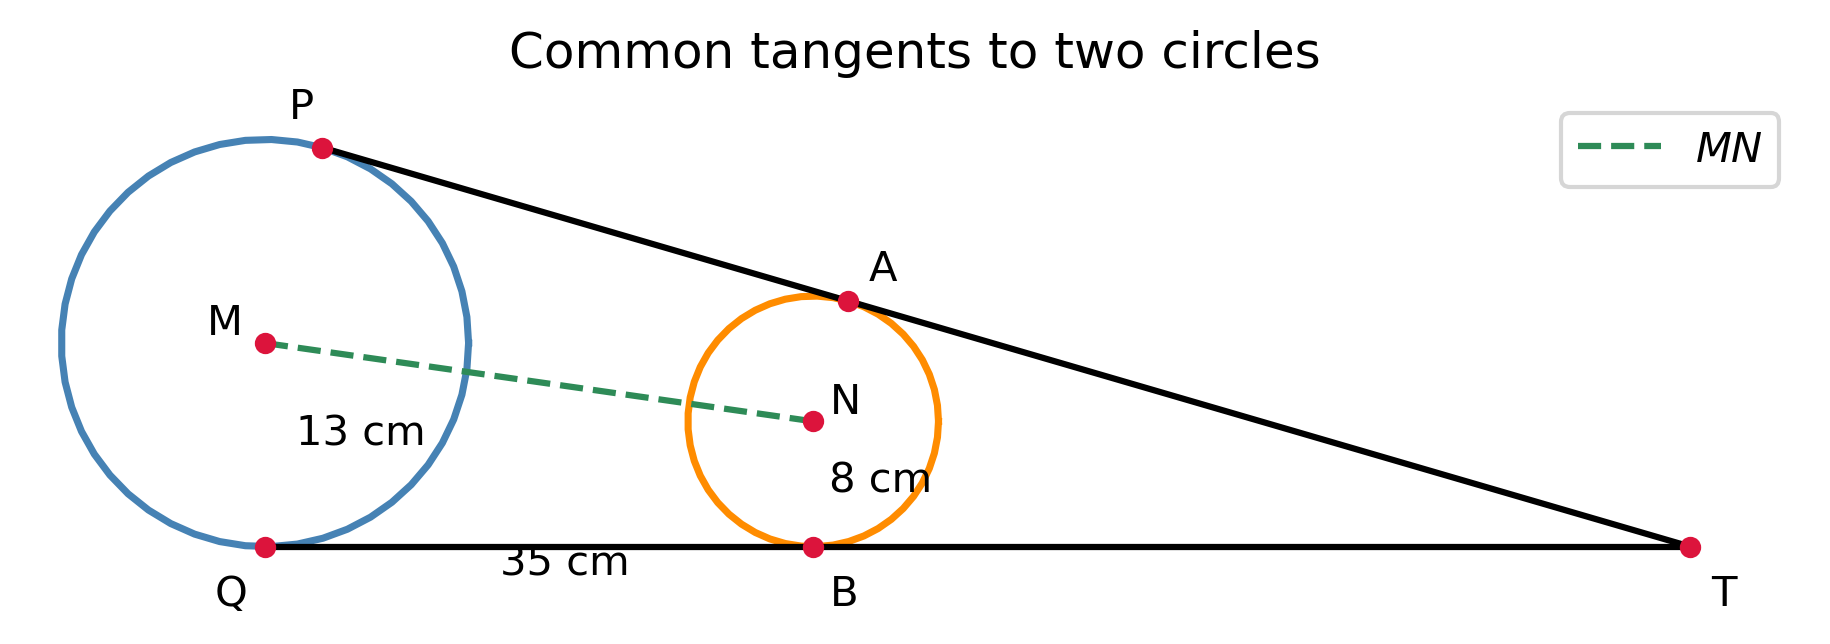
\includegraphics[width=0.38\linewidth]{figs/4.1.33.png}
    \caption{Schematic two-circle tangent configuration.}
\end{figure}
\end{list}

\vspace{0.8em}
\begin{list}{}{\setlength{\leftmargin}{1.15cm}\setlength{\labelwidth}{1.0cm}\setlength{\labelsep}{0.15cm}\setlength{\itemindent}{0pt}\setlength{\listparindent}{0pt}\setlength{\parsep}{0pt}\setlength{\topsep}{0pt}}
\item[4.1.34] A kite is flying $60$ m above the ground. Ravi, on the roof of a house, holds the string straight and sees the kite at an angle of elevation of $30^\circ$. From the bottom of the building, the angle of elevation is $45^\circ$. Find the string length and the height of the roof. Use $\sqrt3=1.73$.

\vspace{0.7em}\par\noindent\textbf{Solution:}

The $45^\circ$ angle from the building's bottom gives a horizontal distance of $60$ m to the kite's vertical projection. From the roof,
\[
\tan30^\circ=\frac{60-h}{60}\quad\Longrightarrow\quad h=60-20\sqrt3\approx25.4\text{ m}.
\]
The string length is
\[
\sqrt{60^2+(20\sqrt3)^2}=40\sqrt3\approx69.2\text{ m}.
\]

The code draws the right-triangle configuration and calculates both lengths.
\begin{lstlisting}[frame=single, basicstyle=\rmfamily, escapeinside={(*@}{@*)}]
(*@\makebox[\dimexpr\linewidth-2\fboxsep-2\fboxrule\relax][c]{codes/4.1.34.py}@*)
\end{lstlisting}
\begin{figure}[H]
    \centering
    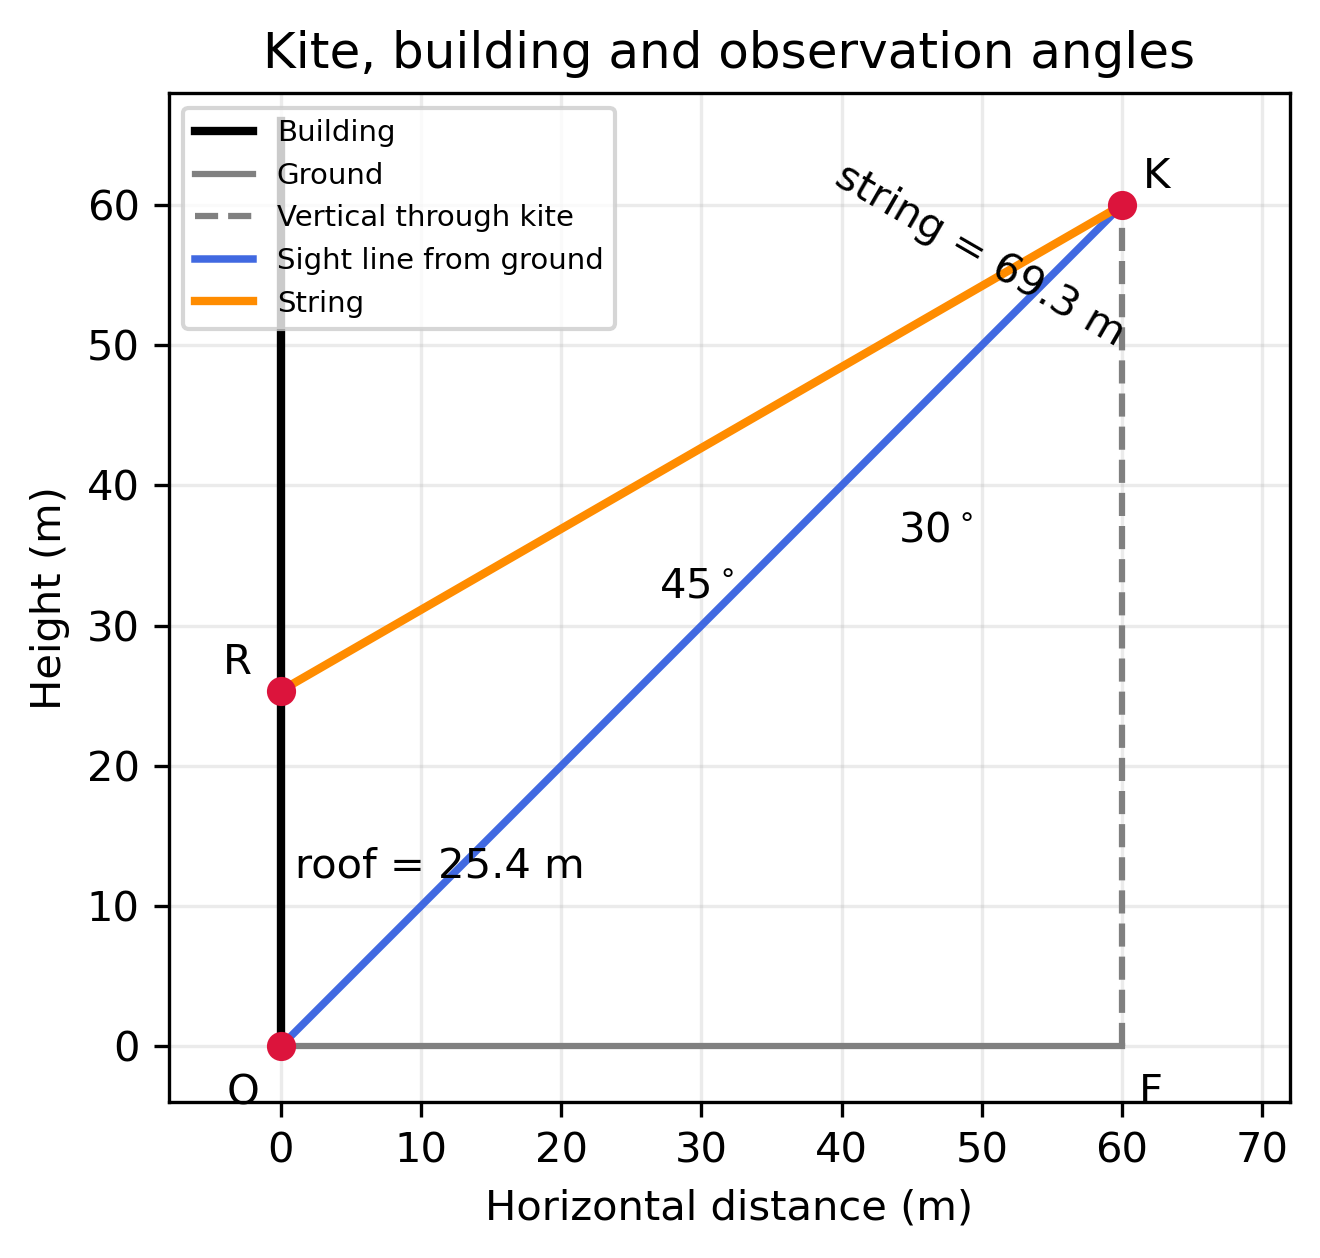
\includegraphics[width=0.40\linewidth]{figs/4.1.34.png}
    \caption{Kite and building geometry, with the two angles of elevation.}
\end{figure}
\end{list}

\vspace{0.8em}
\begin{list}{}{\setlength{\leftmargin}{1.15cm}\setlength{\labelwidth}{1.0cm}\setlength{\labelsep}{0.15cm}\setlength{\itemindent}{0pt}\setlength{\listparindent}{0pt}\setlength{\parsep}{0pt}\setlength{\topsep}{0pt}}
\item[4.1.37] A Kolam pattern has successive dot counts $4,8,12,\ldots$. Find (i) the A.P.'s first term and common difference, (ii) its $n$th term, and (iii)(a) the number of squares formed with $220$ dots, or (b) whether $100$ dots can form a whole number of squares.

\vspace{0.7em}\par\noindent\textbf{Solution:}

The counts form an A.P. with $a=4$, $d=4$, and $a_n=4n$. The total is $S_n=2n(n+1)$. For $220$ dots, $2n(n+1)=220$, so $n=10$. For $100$ dots, $n(n+1)=50$ has no integer solution; hence a whole number of squares cannot be completed.

The C program calculates the A.P. terms and checks both totals.
\begin{lstlisting}[frame=single, basicstyle=\rmfamily, escapeinside={(*@}{@*)}]
(*@\makebox[\dimexpr\linewidth-2\fboxsep-2\fboxrule\relax][c]{codes/4.1.37.c}@*)
\end{lstlisting}
\end{list}

\vspace{0.8em}
\begin{list}{}{\setlength{\leftmargin}{1.15cm}\setlength{\labelwidth}{1.0cm}\setlength{\labelsep}{0.15cm}\setlength{\itemindent}{0pt}\setlength{\listparindent}{0pt}\setlength{\parsep}{0pt}\setlength{\topsep}{0pt}}
\item[4.1.38] On a Cartesian map of Jaipur, Rambagh Palace is the origin. The locations are $A=(-4,2)$ (Rajasthan High Court), $B=(4,-4)$ (Birla Mandir), $C=(4,3)$ (Heera Bagh), and $D=(-5,-2)$ (Amar Jawan Jyoti). Find: (i) the daily distance from Heera Bagh to the court and back; (ii) the ratio in which the $x$-axis divides $AD$; (iii)(a) whether Birla Mandir is equidistant from Heera Bagh and Amar Jawan Jyoti, or (b) show using the section formula that $A,O,B$ are not collinear.

\vspace{0.7em}\par\noindent\textbf{Solution:}

(i) $AC=\sqrt{(4+4)^2+(3-2)^2}=\sqrt{65}$, so the round trip is $2\sqrt{65}\approx16.12$ map units.\\
(ii) $A$ and $D$ have $y$-coordinates $2$ and $-2$, so the $x$-axis bisects $AD$ in the ratio $1:1$.\\
(iii)(a) $BC=7$, while $BD=\sqrt{9^2+2^2}=\sqrt{85}$. These are unequal, so Birla Mandir is not equidistant from $C$ and $D$.\\
Alternatively, for (iii)(b), the point dividing $AB$ in the ratio $1:1$ is, by the section formula, $\bigl(\frac{-4+4}{2},\frac{2-4}{2}\bigr)=(0,-1)$. Since $A$ and $B$ have opposite $x$-coordinates, any point on $AB$ with $x=0$ must divide it in ratio $1:1$. This point is not $O=(0,0)$, so $A,O,B$ are not collinear.

The code plots the four locations, origin, and the segments used in the answers.
\begin{lstlisting}[frame=single, basicstyle=\rmfamily, escapeinside={(*@}{@*)}]
(*@\makebox[\dimexpr\linewidth-2\fboxsep-2\fboxrule\relax][c]{codes/4.1.38.py}@*)
\end{lstlisting}
\begin{figure}[H]
    \centering
    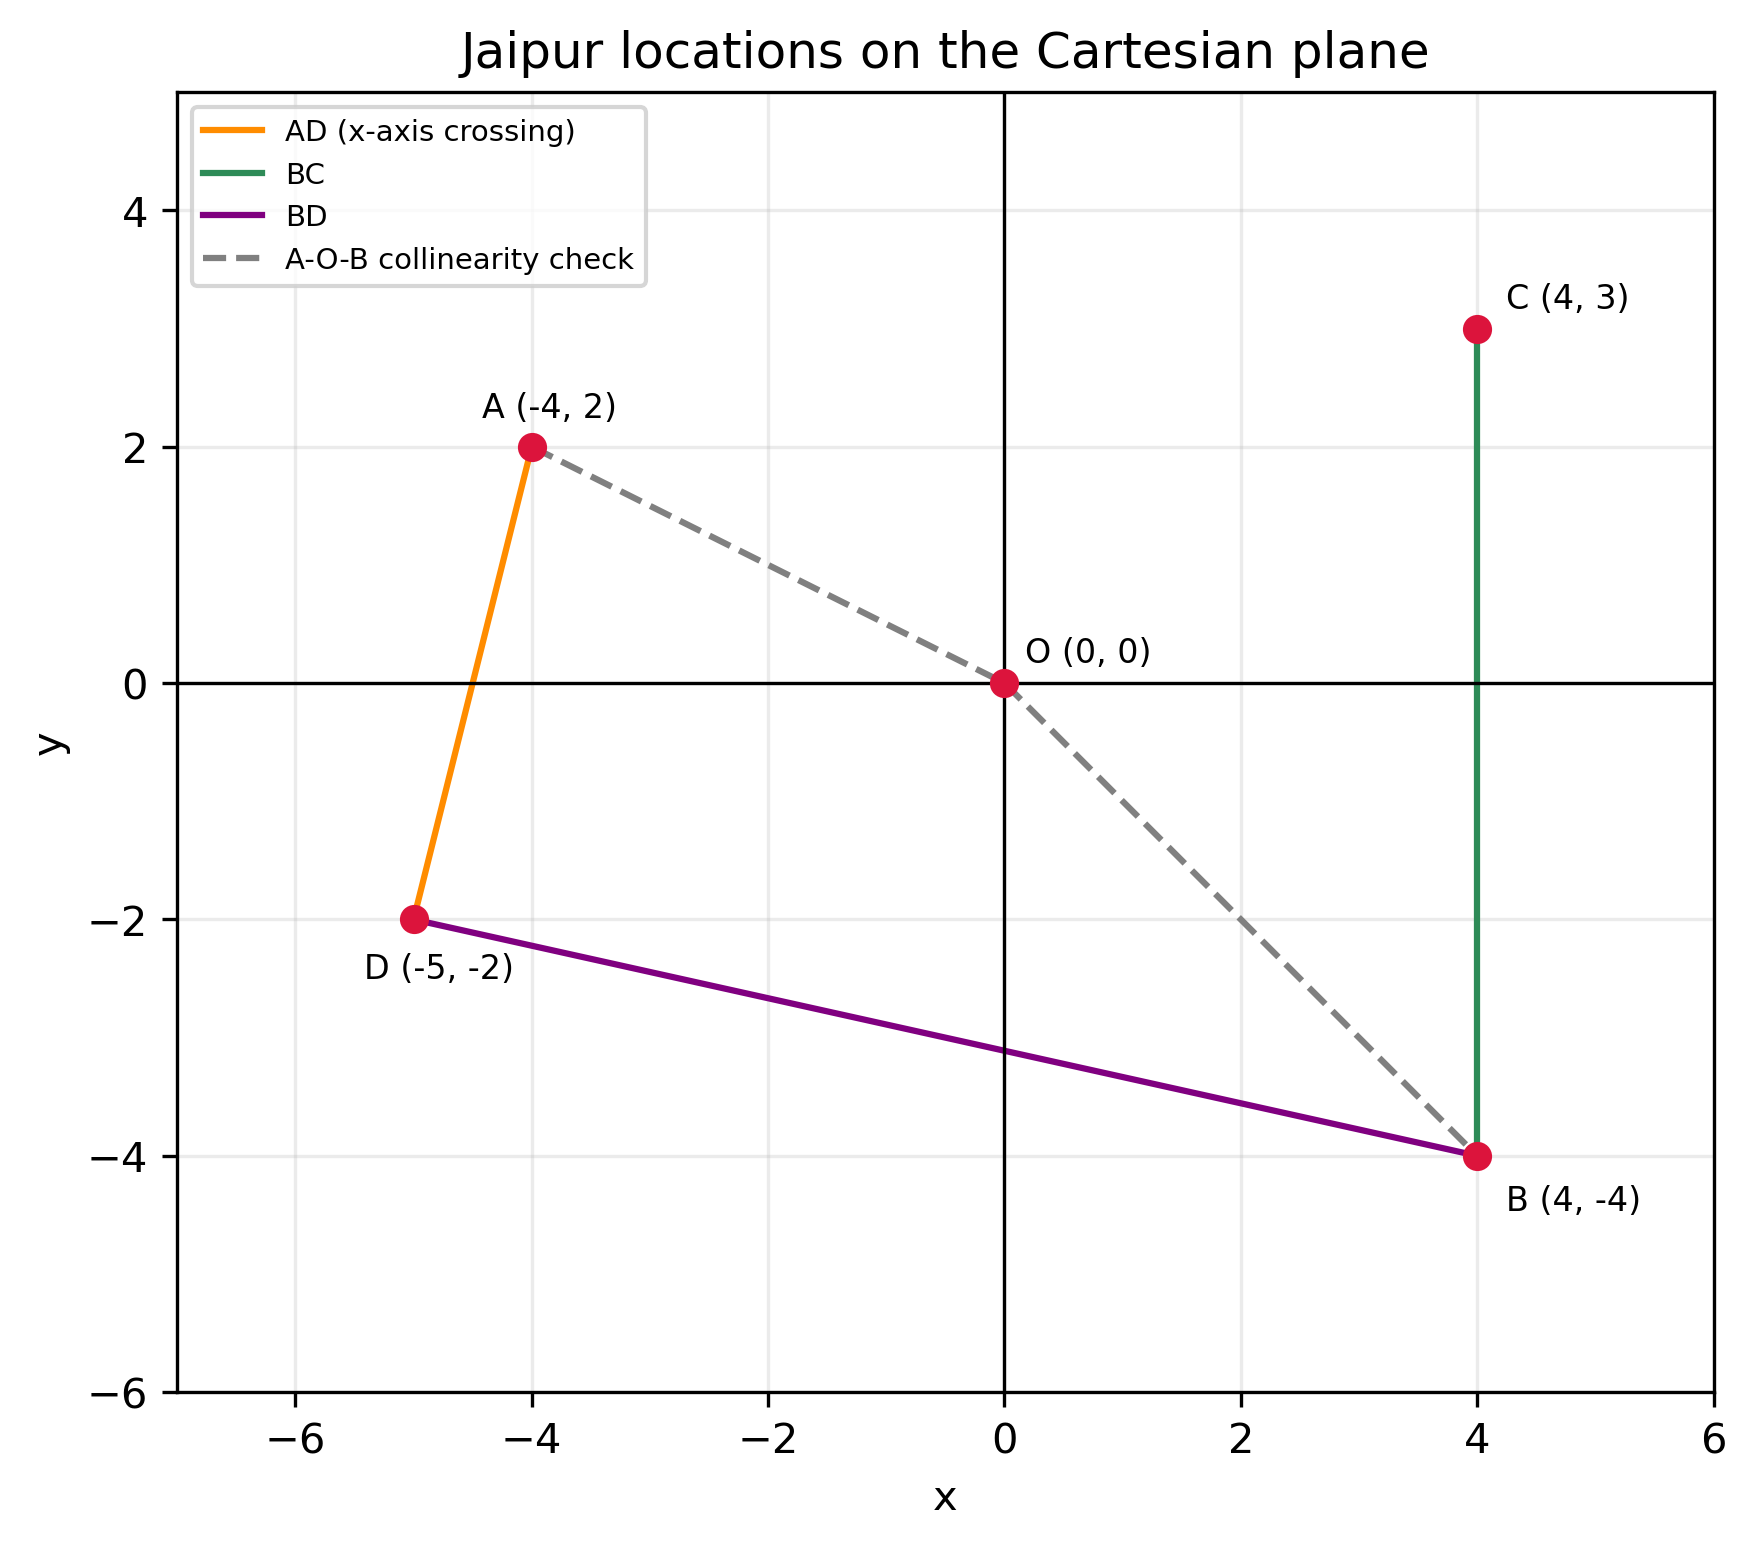
\includegraphics[width=0.48\linewidth]{figs/4.1.38.png}
    \caption{Jaipur locations plotted on the Cartesian plane.}
\end{figure}
\end{list}
\end{document}
